\documentclass[fleqn,reqno,10pt,draft]{article}


\usepackage[natbib=true,
            style=authoryear-comp,
            backend=bibtex,
            sortcites=false,
            maxnames=2,
            doi=false,
            url=false]{biblatex}
% \bibliography{../helpers/MyRefGlobal}
\bibliography{paper}

\usepackage[final,            % override "draft" which means "no nothing"
            colorlinks,       % rather than outlining them in boxes
            linkcolor=gray,   % override truly awful colour choices
            citecolor=gray,   %   (ditto)
            urlcolor=gray,    %   (ditto)
            plainpages=false, % to overcome complaints with multiple
            pdfpagelabels,    % multiple page 1-s due to preface
            hypertexnames=false % solves warning, but interferes with
                                % index and \autoref apparently
            ]{hyperref}


\usepackage{amsmath}            % Formeln
\usepackage{amsfonts}           % Fonts for Formulas
\usepackage{amssymb}
\usepackage[final]{graphicx}
\usepackage{booktabs}
\usepackage{enumerate}
\usepackage{lipsum}
\usepackage{txfonts} % for strict implication symbols
\usepackage{soul}
\usepackage{relsize} % provides command \relsize{+/-x} for relative
                     % font size changes
\usepackage[german,english]{babel}
\usepackage[utf8]{inputenc}
\usepackage[T1]{fontenc} 
\usepackage{subfig}
\usepackage{xypic}
\usepackage{url}
\usepackage{tikz}
\usetikzlibrary{arrows,shapes,automata,backgrounds,petri,fit,decorations.pathmorphing}
\usepackage{refcount}
\usepackage{xspace} % for \xspace in definition of acronyms etc.
\usepackage{attrib} % for right-aligned references at the end of
                    % quotes; part of Frankenstein bundle, but 
\renewcommand\PreTrib {}   % overwrite these commands, from attrib.sty
\renewcommand\PostTrib {}  % to suppress additional brackets around
                           % attributions

\usepackage{pgfplots}


\usepackage{../helpers/gb4e_micha}
\usepackage{../helpers/proofing}

\usepackage{../helpers/mycommands}
% \usepackage{../helpers/myenvironments}

\usepackage[]{svninfo}
\usepackage{subfig}

%%%% Additional Macros

\newcommand{\lit}{\acro{lit}}
\newcommand{\glb}{\acro{glb}}
\newcommand{\loc}{\acro{loc}}

\newcommand{\as}{\acro{as}}
\renewcommand{\es}{\acro{es}}
\renewcommand{\AE}{\as}
\newcommand{\GE}{\es}

\newcommand{\lc}{\acro{lc}}
\newcommand{\ec}{\acro{ec}}
\newcommand{\LC}{\lc}
\newcommand{\EC}{\ec}

\newcommand{\exh}{\ensuremath{\mathrm{Exh}}}
\newcommand{\alt}{\ensuremath{\mathrm{Alt}}}


%%%% Document

\title{Scalar Items in Embedded Position: {A}n Experimental Revisit}
\author{Fabian Schlotterbeck, Michael Franke and Petra Augurzky}
\date{}

\begin{document}
\maketitle



\begin{abstract}
  \dots make concrete \dots
\end{abstract}

\tableofcontents

\svnInfo $Id$

\section{Introduction}
\label{sec:introduction}

The existential quantifier \emph{some} is usually assumed to receive a
semantic interpretation similar to logical $\exists$, so that the
sentence \emph{Some boys cried} is literally true in a situation where
all boys cried. But it is also usually considered to be a
\mymark{scalar item} in that its use invites comparison with (at
least) the semantically stronger universal quantifier \emph{all}
\citep[c.f.][]{Horn1972:On-the-Semantic,Gazdar1979:Pragmatics:-Imp,AtlasLevinson1981}. This
comparison can lead to an upper-bounding meaning enrichment, e.g.,
when an utterance of (\ref{bsp:Plain-SI-Target}) is taken to invite
the inference in (\ref{bsp:Plain-SI-Implicature}).

\begin{exe}
  \ex \label{bsp:Plain-SI}
    \begin{xlist}
      \ex \label{bsp:Plain-SI-Target} Hans solved some of the
        problems.
      \ex \label{bsp:Plain-SI-Implicature} $\implicates$ Hans solved
        some but not all of the problems.
      \ex \label{bsp:Plain-SI-Alternative} Hans solved all of the problems.
    \end{xlist}
\end{exe}

\noindent The classical explanation of this inference, following the
pioneering work of \citet{Grice1975:Logic-and-Conve} \citep[see][for
recent overview]{Geurts2010:Quantity-Implic}, is that
(\ref{bsp:Plain-SI-Implicature}) is a pragmatic inference, a so-called
\emph{quantity implicature}, derived by an abductive inference as the
best explanation of why an informed, knowledgable and cooperative
speakers have uttered (\ref{bsp:Plain-SI-Target}) when they could also
have uttered the semantically stronger and relevant
(\ref{bsp:Plain-SI-Alternative}).


% If this upper-bounding inference would occur often and
% systematically enough, then it may well be that also embedded
% occurrences of \emph{some} get enriched, in some fashion or other, to
% contribute the enriched meaning \emph{some but not all} also under the
% scope of other logical operators.
% Indeed, even
% \citeauthor{Grice1975:Logic-and-Conve} envisaged this possibility when
% he wrote: ``It may not be impossible for what starts life, so to
% speak, as a conversational implicature to become conventionalized''
% \citep[p.58]{Grice1975:Logic-and-Conve}.


This paper deals with the interpretation of two types of sentences,
where the scalar item \emph{some} occurs in the scope of other logical
operators. In \as-sentences (short for \textsc{All-Some}) as in (\ref{bsp:AE})
the scalar item \emph{some} is embedded under universal quantifier
\emph{all}. In \es-sentences (short for \textsc{ExactlyOne-Some}) like (\ref{bsp:GE}) \emph{some} takes
scope under the non-monotonic quantifier \emph{exactly
  one}.\dn{explain what non-monotonic means?  here or later?}
According to current pragmatic theory, there are at least three
relevant candidate readings for \as- and \es-sentences: (i) a
\emph{literal reading} like in (\ref{bsp:AE-Literal}) and
(\ref{bsp:GE-Literal}) where \emph{some} has only its literal meaning;
(ii) a \emph{global reading} like in (\ref{bsp:AE-Global}) and
(\ref{bsp:GE-Global}) where, according to Gricean intuition, we enrich
utterances of (\ref{bsp:AE}) and (\ref{bsp:GE}) with the negation of
alternative utterances of the corresponding sentences
(\ref{bsp:AE-Alternative}) and (\ref{bsp:GE-Alternative}) where
\emph{some} is replaced by \emph{all}; and also (iii) a \emph{local
  reading} like in (\ref{bsp:AE-Local}) and (\ref{bsp:GE-Local}) where
\emph{some} is interpreted as \emph{some but not all} in the scope of
the embedding quantifier.


\begin{exe}
  \ex \label{bsp:AE} \mymark{All} of the students read {\mymark{some}} of the
  papers. \hfill{(\as)}

  \begin{xlist}
  \ex \label{bsp:AE-Literal} \mymark{All} of the students read
    {\mymark{some and maybe all}} of the papers. \hfill (\as-\lit)
  \ex \label{bsp:AE-Global}
    \mymark{All} of the students read \mymark{some and maybe all} 
    and  \hfill (\as-\glb)\\
    it's not the case that \mymark{all} of the students read \mymark{all} of the papers.
  \ex \label{bsp:AE-Local}
    \mymark{All} of the students read {\mymark{some  but not all}} of the
    papers. \hfill (\as-\loc)
  \end{xlist}
\end{exe}

\begin{exe}
\ex  \label{bsp:GE} \mymark{Exactly one} of the students read {\mymark{some}} of the
  papers. \hfill{(\es)}

  \begin{xlist}
  \ex \label{bsp:GE-Literal} \mymark{Exactly one} of the students read
    {\mymark{some and maybe all}} of the papers. \hfill (\es-\lit)
  \ex \label{bsp:GE-Global}
    \mymark{Exactly one} of the students read \mymark{some and maybe all} 
    and  \hfill (\es-\glb)\\
    it's not the case that \mymark{exactly one} of the students read \mymark{all} of the papers.
  \ex \label{bsp:GE-Local}
    \mymark{Exactly one} of the students read {\mymark{some  but not all}} of the
    papers. \hfill (\es-\loc)
  \end{xlist}
\end{exe}


\begin{exe}
\ex \label{bsp:AE-Alternative} \mymark{All} of the students read
  {\mymark{all}} of the papers. 

\ex \label{bsp:GE-Alternative} \mymark{Exactly one} of the students
  read {\mymark{all}} of the papers.
\end{exe}

% Section~\ref{sec:get-know-your} will discuss these readings
% in more detail, showing that all three readings of each sentence are
% distinct but logically dependent on each other in interesting ways.

\noindent Given this relative abundance of theoretically conceivable
readings, two interlocked empirical questions arise:
\begin{enumerate}[Q1:]
\item which of these three
conceivable readings are available to na\"{i}ve subjects; and
\item which of the available readings are preferred.\fn{It may
    ultimately be impossible to keep unavailability and strong
    dispreference strictly apart. For our purposes this is not
    important. Every time we speak of availability, the so-inclined
    reader may think of non-negligible preference.}
\end{enumerate}
Addressing these questions empirically is relevant because they lie at
the heart of the current debate about the exact location and nature of
the interface between semantics and pragmatics. The controversy
concerns the question to what extent the upper-bounding inference from
\emph{some} to \emph{some but not all} is conventionalized within the
compositional computation of semantic values. For that matter, it is
particularly relevant to assess the availability and relative
preference of local readings. (Section~\ref{sec:theories-predictions}
will discuss the relevant theoretical positions and the significance
of alleged local readings in more detail.)

% Firstly, there are \mymark{pragmatic traditionalists} who seek to
% conserve the spirit of \citeauthor{Grice1975:Logic-and-Conve}'s
% (\citeyear{Grice1975:Logic-and-Conve}) original ideas as much as
% possible
% \citep[e.g.][]{Spector2006:Scalar-Implicat,Sauerland2004:Scalar-Implicat,Russell2006:Against-Grammat,vanRooijSchulz:ExhaustiveInterpretation,Geurts2010:Quantity-Implic,Franke2011:Quantity-Implic}. Traditionalists
% acknowledge the existence of global readings, but might consider local
% readings either unavailable or a beast distinct from scalar
% implicatures. An often phrased intuition of the traditionalists is
% that local readings, since they are special kinds of inferences,
% require special intonation, in particular emphatic stress on the
% scalar item.\dn{give references}

% Opposed to that is the camp of \mymark{lexical conventionalists}
% \citep[e.g.][]{LevinsonPresumptiveMeanings2000,Chierchia:2004_ScalarImplicatures}
% who maintain that scalar \emph{some} is lexically ambiguous between
% the standard logical meaning \emph{some and maybe all} and the
% upper-bounded meaning \emph{some but not all}. As the latter is
% considered a default, lexical conventionalism has no problem
% accounting for local readings, and in fact would consider these the
% preferred readings. 

% Thirdly and finally, there is the camp of \mymark{grammaticalists} who
% defend that the distribution of upper-bounded readings of \emph{some}
% is best explained by postulating a silent operator, akin to the
% meaning of the particle \emph{only}
% \citep{Chierchia2006:Broaden-Your-Vi,Fox2007:Free-Choice-and,Magri2011:Another-Argumen,Sauerland2012:The-Computation,ChierchiaFox2008:The-Grammatical,Chierchia2012:FC-Nominals-and}. According
% to the grammatical view, this silent operator may be applied in
% compositional semantics also in the scope of other logical operators,
% but, so as not to overgenerate readings, the availability of readings
% is constraint by the \emph{strongest meaning hypothesis}
% \citep{DalrympleKanazawa1998:Reciprocal-Expr}. Grammaticalist theories
% predict that all three types of readings are available. Moreover,
% according to the grammatical view, the local reading is preferred for
% \as-sentences, while the global one is preferred for
% \es-sentences. (More precisely, as we will see
% Section~\ref{sec:theories-predictions}, depending on the variant of
% the strongest meaning hypothesis employed, either the global reading
% is predicted to be preferred for \es-sentences, or the global and the
% local reading are predicted to be equally preferred.)

A number of empirical studies have already examined the availability
of readings for \as- and \es-sentences
\citep[e.g.][]{GeurtsPouscoulous2009:Embedded-Implic,CliftonDube2010:Embedded-Implic,ChemlaSpector2010:Experimental-Ev}. However,
results have not been as clear-cut as one might have hoped for: for
instance, the available empirical evidence is inconclusive as to
whether local readings exist \citep[see also][for related
discussion]{Tielvan-Tiel2012:Embedded-Scalar} and do not clearly
address all preference relations between readings relevant to
distinguish between theoretical positions. In the following we will
argue that these heterogeneous results are partly due to the specific
tasks used in previous studies, i.e., complexity differences in
variants of the picture-verification paradigm.
% We hypothesized that previous studies might be
% insufficiently informative because of the focus on (variants of) a
% picture-verification paradigm.\dn{relate to Bob van Tiel's work} The
% problem is that in order to test the availability of different
% candidate meanings different pictures have to be presented, so that
% effects of pictorial complexity or stereotypicality could never be
% ruled out entirely.
Moreover, previous studies have only accumulated limited evidence
pertaining to the second question that may help decide between
theoretical positions, namely which of the attested readings subjects
prefer. Finally, previous studies presented target sentences
visually. But as it is often argued that intonational stress on an
embedded scalar item can favor a local reading
\citep[e.g.][]{Horn2006:The-Border-Wars,Geurts2009:Scalar-Implicat,ChemlaSpector2010:Experimental-Ev,Geurts2010:Quantity-Implic,Tielvan-Tiel2012:Embedded-Scalar},
it seems important to present target sentences auditorily, so as to be
able to control for effects of ``silent intonation'' that subjects may
apply when reading a sentence (see Bader 1998, Fodor 2000)\dn{provide
  references}.

In reaction to this situation, we therefore presented sentence
material auditorily and also employed a different kind of visual
presentation of the pictorial material: subjects were presented with
pictures that were initially covered and could incrementally be
uncovered at the subjects' request; at each step of uncovering,
subjects had to decide whether they could already give a truth-value
judgement or needed more information (Comry ????)\dn{insert
  references}. This way we obtained behavioral data that is both
indicative of the reading subjects assumed and independent of the
complexity of the visual stimulus. At the same time, we hypothesized
that the incremental nature of this task would shed light on the
preferences over readings, because the temporal distribution of
truth-value judgments would give away which reading subjects were
waiting to evaluate, so to speak. Adding to previous studies, we
therefore made sure that our method is able to reveal information
about preferential readings by including ambiguous test items like
(\ref{bsp:target-related-filler}) which are known to preferentially
receive the late-closure reading in
(\ref{bsp:target-related-filler-LC}) and not the dispreferred, but
attested early-closure reading (\ref{bsp:target-related-filler-EC})
(Frazier 1987 XYZ).\dn{insert proper references}
\begin{exe}
\ex \label{bsp:target-related-filler} The letter is connected with circles and squares with
  suns.
  \begin{xlist}
  \ex \label{bsp:target-related-filler-LC} The letter is connected
    with squares with suns and circles. \hfill (\LC)
  \ex \label{bsp:target-related-filler-EC} The letter is connected
    with circles with suns and squares with suns. \hfill (\EC)
  \end{xlist}
\end{exe}

% \begin{itemize}
% \item Fabian wants to skip the following; Petra wants to enlarge on
%   it; I give first my version, then Petra's
%   \begin{itemize}
%   \item To test whether our method is indeed suitable to detect
%     interpretation preferences, we included ambiguous test items like
%     (\ref{bsp:target-related-filler}) which are known to
%     preferentially receive the late-closure reading in
%     (\ref{bsp:target-related-filler-LC}) and not the dispreferred, but
%     attested early-closure reading
%     (\ref{bsp:target-related-filler-EC}).\dn{insert references to
%       literature on EC-LC processing}

%     \begin{exe}
%     \ex \label{bsp:target-related-filler} The letter is connected with circles and squares with
%       suns.
%       \begin{xlist}
%       \ex \label{bsp:target-related-filler-LC} The letter is connected
%         with squares with suns and circles. \hfill (\LC)
%       \ex \label{bsp:target-related-filler-EC} The letter is connected
%         with circles with suns and squares with suns. \hfill (\EC)
%       \end{xlist}
%     \end{exe}
%   \item To test whether our method is indeed suitable to detect
%     interpretation preferences, we included ambiguous test items like
%     (\ref{bsp:target-related-filler}) which have been repeatedly shown
%     to exhibit preferences in previous studies. We thus included
%     so-called \emph{late-closure structures} in which a propositional
%     phrase can be either attached to the immediately preceding
%     \acro{np} (the ``late-closure'' (\LC) reading as
%     (\ref{bsp:target-related-filler-LC})), or to an
%     \acro{np}-coordination (the ``early-closure'' (\EC) readins as in
%     (\ref{bsp:target-related-filler-EC})). According to principles of
%     structural simplicity, an advantage for the \LC-reading has been
%     repeatedly demonstrated (Frazier 1987 XYZ).\dn{insert proper
%       references}
%     \begin{exe}
%     \ex \label{bsp:target-related-filler} The letter is connected with circles and squares with
%       suns.
%       \begin{xlist}
%       \ex \label{bsp:target-related-filler-LC} The letter is connected
%         with squares with suns and circles. \hfill (\LC)
%       \ex \label{bsp:target-related-filler-EC} The letter is connected
%         with circles with suns and squares with suns. \hfill (\EC)
%       \end{xlist}
%     \end{exe}
%     By including these structures, we intended to control whether
%     dispreferred readings in general were still available to our
%     participants in the specific task used.

% \end{itemize}
% \end{itemize}
 
% To test whether our method is indeed suitable to detect interpretation
% preferences, we included ambiguous test items like
% (\ref{bsp:target-related-filler}) which have been repeatedly shown to
% exhibit preferences in previous studies.
% \begin{exe}
% \ex \label{bsp:target-related-filler} The letter is connected with circles and squares with
%   suns.
%   \begin{xlist}
%   \ex \label{bsp:target-related-filler-LC} The letter is connected
%     with squares with suns and circles. \hfill (\LC)
%   \ex \label{bsp:target-related-filler-EC} The letter is connected
%     with circles with suns and squares with suns. \hfill (\EC)
%   \end{xlist}
% \end{exe}
% Sentence (\ref{bsp:target-related-filler}) is an example of a
% so-called \emph{late-closure structure} in which a propositional
% phrase can be either attached to the immediately preceding \acro{np}
% (the ``late-closure'' (\LC) reading as
% (\ref{bsp:target-related-filler-LC})), or to an \acro{np}-coordination
% (the ``early-closure'' (\EC) readins as in
% (\ref{bsp:target-related-filler-EC})). According to principles of
% structural simplicity, an advantage for the \LC-reading has been
% repeatedly demonstrated (Frazier 1987 XYZ).\dn{insert proper
%   references}

\medskip

\begin{itemize}
\item summarize results
\end{itemize}

The paper is structured as follows. Section~\ref{sec:get-know-your}
elaborates on the three kinds of relevant readings for our target
sentences. Section~\ref{sec:theories-predictions} works out the
different theoretical positions and their predictions about
availability and preference. Section~\ref{sec:previous-studies} recaps
the results of previous studies on this subject, arguing for the need
of a more refined methodology. Section~\ref{sec:design} describes our
experimental design. Section~\ref{sec:results} states our results,
which we discuss in Section~\ref{sec:discussion}.\dn{rephrase
  eventually}

\section{Get to know your readings}
\label{sec:get-know-your}

Three readings are \emph{prima facie} conceivable for the \as- and
\es-sentences in (\ref{bsp:AE}) and (\ref{bsp:GE}). These are
logically dependent in intricate ways.

\paragraph{\as-sentences.}

An \as-sentence like (\ref{bsp:AE}), repeated below, has a literal
reading (\lit) as in (\ref{bsp:AE-Literal}), a global reading (\glb) as in
(\ref{bsp:AE-Global}) and a local reading (\loc) as in (\ref{bsp:AE-Local}).

\begin{exer}{bsp:AE}

  \ex \mymark{All} of the students read {\mymark{some}} of the
  papers. 

  \begin{xlist}
  \ex \mymark{All} of the students read
    {\mymark{some and maybe all}} of the papers. \hfill (\as-\lit)
  \ex
    \mymark{All} of the students read \mymark{some and maybe all} 
    and  \hfill (\as-\glb)\\
    it's not the case that \mymark{all} of the students read \mymark{all} of the papers.
  \ex
    \mymark{All} of the students read {\mymark{some  but not all}} of the
    papers. \hfill (\as-\loc)
  \end{xlist}
\end{exer}

\noindent These readings stand in a strict entailment relation: the
local reading asymmetrically entails the global reading, which
asymmetrically entails the literal reading:
\begin{exe}
  \ex \label{bsp:Entailments-AS} \loc $\subset$ \glb $\subset$ \lit
\end{exe}
\glb entails \lit because, in general, global readings are defined as
the conjunction of the literal reading and the negated
(relevant/feasible) alternative(s) of the to-be-interpreted
utterance. This entailment is asymmetric, because the information that
not all of the students read all of the papers is not entailed by the
literal reading. To see that \loc $\subset$ \glb, notice that the case
where all of the students read some but not all of the papers is a
special case of the case where all of the students read some (and
maybe all), while not all of the students read all of the papers.

Given these entailment relations, there are four kinds of situations,
the names for which we borrow from
\citet{ChemlaSpector2010:Experimental-Ev}, that we can distinguish
based on different truth values for our candidate readings. These are
given in Table~\ref{fig:situations-AE}.
%
\begin{table}
  \centering
  \subfloat[][\as-sentences]{
  \label{fig:situations-AE}
    \begin{tabular}{lccc}
    \toprule
    situation    & \multicolumn{3}{c}{truth value} 
  \\ 
  \cmidrule(r){2-4}
     & \lit & \glb & \loc \\ \midrule
    false   & 0 & 0 & 0 \\
    literal & 1 & 0 & 0 \\
    weak    & 1 & 1 & 0 \\
    strong  & 1 & 1 & 1 \\ \bottomrule
  \end{tabular}
} \qquad \qquad
  \subfloat[][\es-sentences]{
  \label{fig:situations-GS}
  \begin{tabular}{lccc}
    \toprule
    situation    & \multicolumn{3}{c}{truth value} 
  \\ 
  \cmidrule(r){2-4}
    & \textsc{lit} & \textsc{glb} & \textsc{loc} \\ \midrule
    false   & 0 & 0 & 0 \\
    literal & 1 & 0 & 0 \\
    local   & 0 & 0 & 1 \\
    all     & 1 & 1 & 1 \\ \bottomrule
  \end{tabular}
}
\caption{Possible truth-value distributions for readings of \as- and \es-sentences}
\label{tab:situations}
\end{table}
%
Examples of these kinds of situations are given in
Figure~\ref{fig:AS-distinguishing-pics}, where the dots on the right
of each diagram represent students, the dots on the left represent
papers and an arrow from a student to a paper indicates that the
student read the paper.\dn{improve graphics} Notice that other
arrangements of arrows might equally well serve as examples for the
various situations.

\begin{figure}[]
  \centering
  
\subfloat[fig:false][false]{
  \label{fig:false-AE}
  
\begin{tikzpicture}[node distance = 1cm]
        % Nodes

        \node (X-1) {$\Large{\bullet}$};

        \node (X-2) [below of = X-1] {$\Large{\bullet}$};

        \node (X-3) [below of = X-2] {$\Large{\bullet}$};

        \node (Y-1) [right of = X-1, node distance = 2cm]{$\Large{\bullet}$};

        \node (Y-2) [below of = Y-1] {$\Large{\bullet}$};

        \node (Y-3) [below of = Y-2] {$\Large{\bullet}$};

        \node (Y-4) [below of = Y-3] {$\Large{\bullet}$};

        % table added from here

        \node (X-4) [below of = X-3, node distance = 2cm] {};

        \node (table) [right of = X-4] {
          \begin{tabular}{ll}
            \lit & false \\
            \glb & false \\
            \loc & false 
          \end{tabular}};

        % Arrows

        \path [draw=blue,->] (X-1) -> (Y-1);

        \path [draw=blue,->] (X-1) -> (Y-2);


        \path [draw=red,->] (X-3) -> (Y-3);

        \path [draw=red,->] (X-3) -> (Y-4);

      \end{tikzpicture}

}
\subfloat[fig:literal][literal]{
  \label{fig:literal-AE}

  \begin{tikzpicture}[node distance = 1cm]
        % Nodes

        \node (X-1) {$\Large{\bullet}$};

        \node (X-2) [below of = X-1] {$\Large{\bullet}$};

        \node (X-3) [below of = X-2] {$\Large{\bullet}$};

        \node (Y-1) [right of = X-1, node distance = 2cm]{$\Large{\bullet}$};

        \node (Y-2) [below of = Y-1] {$\Large{\bullet}$};

        \node (Y-3) [below of = Y-2] {$\Large{\bullet}$};

        \node (Y-4) [below of = Y-3] {$\Large{\bullet}$};

        % table added from here

        \node (X-4) [below of = X-3, node distance = 2cm] {};

        \node (table) [right of = X-4] {
          \begin{tabular}{ll}
            \lit & true \\
            \glb & false \\
            \loc & false 
          \end{tabular}};

        % Arrows

        \path [draw=blue,->] (X-1) -> (Y-1);

        \path [draw=blue,->] (X-1) -> (Y-2);

        \path [draw=blue,->] (X-1) -> (Y-3);

        \path [draw=blue,->] (X-1) -> (Y-4);


        \path [draw=black,->] (X-2) -> (Y-1);

        \path [draw=black,->] (X-2) -> (Y-2);

        \path [draw=black,->] (X-2) -> (Y-3);

        \path [draw=black,->] (X-2) -> (Y-4);



        \path [draw=red,->] (X-3) -> (Y-1);

        \path [draw=red,->] (X-3) -> (Y-2);

        \path [draw=red,->] (X-3) -> (Y-3);

        \path [draw=red,->] (X-3) -> (Y-4);

      \end{tikzpicture}

}
\subfloat[fig:weak][weak]{
  \label{fig:weak}

\begin{tikzpicture}[node distance = 1cm]
        % Nodes

        \node (X-1) {$\Large{\bullet}$};

        \node (X-2) [below of = X-1] {$\Large{\bullet}$};

        \node (X-3) [below of = X-2] {$\Large{\bullet}$};

        \node (Y-1) [right of = X-1, node distance = 2cm]{$\Large{\bullet}$};

        \node (Y-2) [below of = Y-1] {$\Large{\bullet}$};

        \node (Y-3) [below of = Y-2] {$\Large{\bullet}$};

        \node (Y-4) [below of = Y-3] {$\Large{\bullet}$};

        % table added from here

        \node (X-4) [below of = X-3, node distance = 2cm] {};

        \node (table) [right of = X-4] {
          \begin{tabular}{ll}
            \lit & true \\
            \glb & true \\
            \loc & false 
          \end{tabular}};

        % Arrows

        \path [draw=blue,->] (X-1) -> (Y-1);

        \path [draw=blue,->] (X-1) -> (Y-2);


        \path [draw=black,->] (X-2) -> (Y-1);

        \path [draw=black,->] (X-2) -> (Y-2);

        \path [draw=black,->] (X-2) -> (Y-3);

        \path [draw=black,->] (X-2) -> (Y-4);


        \path [draw=red,->] (X-3) -> (Y-3);

        \path [draw=red,->] (X-3) -> (Y-4);

      \end{tikzpicture}


}
\subfloat[fig:strong][strong]{
  \label{fig:strong}

\begin{tikzpicture}[node distance = 1cm]
        % Nodes

        \node (X-1) {$\Large{\bullet}$};

        \node (X-2) [below of = X-1] {$\Large{\bullet}$};

        \node (X-3) [below of = X-2] {$\Large{\bullet}$};

        \node (Y-1) [right of = X-1, node distance = 2cm]{$\Large{\bullet}$};

        \node (Y-2) [below of = Y-1] {$\Large{\bullet}$};

        \node (Y-3) [below of = Y-2] {$\Large{\bullet}$};

        \node (Y-4) [below of = Y-3] {$\Large{\bullet}$};

        % table added from here

        \node (X-4) [below of = X-3, node distance = 2cm] {};

        \node (table) [right of = X-4] {
          \begin{tabular}{ll}
            \lit & true \\
            \glb & true \\
            \loc & true 
          \end{tabular}};

        % Arrows

        \path [draw=blue,->] (X-1) -> (Y-1);

        \path [draw=blue,->] (X-1) -> (Y-2);


        \path [draw=black,->] (X-2) -> (Y-2);

        \path [draw=black,->] (X-2) -> (Y-3);


        \path [draw=red,->] (X-3) -> (Y-3);

        \path [draw=red,->] (X-3) -> (Y-4);

      \end{tikzpicture}



}

  \caption{Distinguishing scenarious for \as-sentences}
  \label{fig:AS-distinguishing-pics}
\end{figure}


\paragraph{\es-sentences.}

The situation for \es-sentences like (\ref{bsp:GE}) is similar but a
little more complicated because the embedding quantifier is
non-monotonic. Again, we consider a literal reading as in
(\ref{bsp:GE-Literal}), repeated below, a global reading as in
(\ref{bsp:GE-Global}) and a local reading as in (\ref{bsp:GE-Local}).

\begin{exer}{bsp:GE}
\ex \mymark{Exactly one} of the students read {\mymark{some}} of the
  papers.

  \begin{xlist}
  \ex \mymark{Exactly one} of the students read
    {\mymark{some and maybe all}} of the papers. \hfill (\es-\lit)
  \ex 
    \mymark{Exactly one} of the students read \mymark{some and maybe all} 
    and  \hfill (\es-\glb)\\
    it's not the case that \mymark{exactly one} of the students read \mymark{all} of the papers.
  \ex 
    \mymark{Exactly one} of the students read {\mymark{some  but not all}} of the
    papers. \hfill (\es-\loc)
  \end{xlist}
\end{exer}

\noindent Entailment relations in this case are non-linear:
\begin{exe}
  \ex \label{bsp:Entailments-GE}       \lit\ $\supset$ \glb\ $\color{mycol}{\subset}$ \loc 
    % \hspace{1cm} and \hspace{1cm}  \lit\ $\not \supset$ \loc
\end{exe}
By definition of global readings $\glb$ entails $\lit$. This
entailment is asymmetric because the extra information that it is not
the case that exactly one student read all of the papers is not
entailed by the literal reading (\ref{bsp:GE-Literal}). However,
unlike for \as-sentences, \loc is not stronger than \glb, but
asymmetrically entailed by the latter. To see this, notice that the
global reading is equivalent to:

\begin{exe}
  \exp{bsp:GE-Global} \mymark{Exactly one} of the students read \mymark{some but not
    all} and \\
  \mymark{everybody else} read \mymark{none} of the papers.
\end{exe}

\noindent Finally, \loc and \lit are logically independent: all
possible combinations of truth-values for \loc and \lit are possible.

Given these entailment relations, there are again four different
situations corresponding to the four possible distributions of truth
values for candidate readings. These are given in
Table~\ref{fig:situations-GS} and named following
\citet{ChemlaSpector2010:Experimental-Ev}. Examples for each situation
are given in Figure~\ref{fig:ES-distinguishing-pics}.

\begin{figure}[]
  \centering
  
\subfloat[fig:false][false]{
  \label{fig:false-GE}

  \begin{tikzpicture}[node distance = 1cm]
        % Nodes

        \node (X-1) {$\Large{\bullet}$};

        \node (X-2) [below of = X-1] {$\Large{\bullet}$};

        \node (X-3) [below of = X-2] {$\Large{\bullet}$};

        \node (Y-1) [right of = X-1, node distance = 2cm]{$\Large{\bullet}$};

        \node (Y-2) [below of = Y-1] {$\Large{\bullet}$};

        \node (Y-3) [below of = Y-2] {$\Large{\bullet}$};

        \node (Y-4) [below of = Y-3] {$\Large{\bullet}$};

        % table added from here

        \node (X-4) [below of = X-3, node distance = 2cm] {};

        \node (table) [right of = X-4] {
          \begin{tabular}{ll}
            \lit & false \\
            \glb & false \\
            \loc & false 
          \end{tabular}};


        % Arrows

        \path [draw=blue,->] (X-1) -> (Y-1);

        \path [draw=blue,->] (X-1) -> (Y-2);


        \path [draw=red,->] (X-3) -> (Y-3);

        \path [draw=red,->] (X-3) -> (Y-4);

      \end{tikzpicture}


}
\subfloat[fig:literal][literal]{
  \label{fig:literal-GE}

      \begin{tikzpicture}[node distance = 1cm]
        % Nodes

        \node (X-1) {$\Large{\bullet}$};

        \node (X-2) [below of = X-1] {$\Large{\bullet}$};

        \node (X-3) [below of = X-2] {$\Large{\bullet}$};

        \node (Y-1) [right of = X-1, node distance = 2cm]{$\Large{\bullet}$};

        \node (Y-2) [below of = Y-1] {$\Large{\bullet}$};

        \node (Y-3) [below of = Y-2] {$\Large{\bullet}$};

        \node (Y-4) [below of = Y-3] {$\Large{\bullet}$};

        % table added from here

        \node (X-4) [below of = X-3, node distance = 2cm] {};

        \node (table) [right of = X-4] {
          \begin{tabular}{ll}
            \lit & true \\
            \glb & false \\
            \loc & false 
          \end{tabular}};

        % Arrows

        \path [draw=black,->] (X-2) -> (Y-1);

        \path [draw=black,->] (X-2) -> (Y-2);

        \path [draw=black,->] (X-2) -> (Y-3);

        \path [draw=black,->] (X-2) -> (Y-4);

      \end{tikzpicture}

}
\subfloat[fig:local][local]{
  \label{fig:local}

            \begin{tikzpicture}[node distance = 1cm]
        % Nodes

        \node (X-1) {$\Large{\bullet}$};

        \node (X-2) [below of = X-1] {$\Large{\bullet}$};

        \node (X-3) [below of = X-2] {$\Large{\bullet}$};

        \node (Y-1) [right of = X-1, node distance = 2cm]{$\Large{\bullet}$};

        \node (Y-2) [below of = Y-1] {$\Large{\bullet}$};

        \node (Y-3) [below of = Y-2] {$\Large{\bullet}$};

        \node (Y-4) [below of = Y-3] {$\Large{\bullet}$};

        % table added from here

        \node (X-4) [below of = X-3, node distance = 2cm] {};

        \node (table) [right of = X-4] {
          \begin{tabular}{ll}
            \lit & false \\
            \glb & false \\
            \loc & true 
          \end{tabular}};

        % Arrows

        \path [draw=blue,->] (X-1) -> (Y-1);

        \path [draw=blue,->] (X-1) -> (Y-2);

        \path [draw=blue,->] (X-1) -> (Y-3);

        \path [draw=blue,->] (X-1) -> (Y-4);



        \path [draw=black,->] (X-2) -> (Y-2);

        \path [draw=black,->] (X-2) -> (Y-3);

        \path [draw=black,->] (X-2) -> (Y-4);



        \path [draw=red,->] (X-3) -> (Y-1);

        \path [draw=red,->] (X-3) -> (Y-2);

        \path [draw=red,->] (X-3) -> (Y-3);

        \path [draw=red,->] (X-3) -> (Y-4);

      \end{tikzpicture}

}
\subfloat[fig:all][all]{
  \label{fig:all}

      \begin{tikzpicture}[node distance = 1cm]
        % Nodes

        \node (X-1) {$\Large{\bullet}$};

        \node (X-2) [below of = X-1] {$\Large{\bullet}$};

        \node (X-3) [below of = X-2] {$\Large{\bullet}$};

        \node (Y-1) [right of = X-1, node distance = 2cm]{$\Large{\bullet}$};

        \node (Y-2) [below of = Y-1] {$\Large{\bullet}$};

        \node (Y-3) [below of = Y-2] {$\Large{\bullet}$};

        \node (Y-4) [below of = Y-3] {$\Large{\bullet}$};

        % table added from here

        \node (X-4) [below of = X-3, node distance = 2cm] {};

        \node (table) [right of = X-4] {
          \begin{tabular}{ll}
            \lit & true \\
            \glb & true \\
            \loc & true 
          \end{tabular}};

        % Arrows

        \path [draw=blue,->] (X-1) -> (Y-1);

        \path [draw=blue,->] (X-1) -> (Y-2);

      \end{tikzpicture}

}

  \caption{Distinguishing scenarious for \es-sentences}
  \label{fig:ES-distinguishing-pics}

\end{figure}




\section{Theories and predictions}
\label{sec:theories-predictions}

We consider three main theoretical positions which make different
predictions about the readings of \as- and \es-sentences
\citep[c.f.][for
overview]{Horn2006:The-Border-Wars,Geurts2010:Quantity-Implic,Sauerland2012:The-Computation}. We
will refer to these here as \mymark{traditionalism},
\mymark{conventionalism} and \mymark{grammaticalism} and treat each
one in turn. Since there is some leeway in assessing the predictions
for some of these positions (depending on which of several reasonable
additional assumptions we should adopt), we will distinguish different
varieties of each position. For convenience, the predictions of each
(variety of each) position are also summarized in
Table~\ref{tab:predictions} at the end of this section.\dn{micha says:
I'll leave all the varieties in here until we know which ones we need
and which ones we don't need}

\subsection{Traditionalism}
\label{sec:traditionalism}

We refer to traditionalism as traditionalism because of its
conservative stance towards Grice's original theory of conversational
implicatures \citep{Grice1975:Logic-and-Conve}. Many author's have
defended traditionalist positions in this sense. Of the more recent
literature, we would consider as traditionalist, among others,
contributions by \citet{Spector2006:Scalar-Implicat},
\citet{Sauerland2004:Scalar-Implicat},
\citet{Russell2006:Against-Grammat},
\citet{vanRooijSchulz:ExhaustiveInterpretation},
\citet{Geurts2010:Quantity-Implic} or
\citet{Franke2011:Quantity-Implic}.

According to Grice, conversational implicatures, of which quantity
implicatures are a special case, are to be thought of as
rationalizations of speaker behavior. Central in this reasoning is the
assumption that the speaker's behavior is efficient (if not optimal)
and goal-oriented. Usually, the assumed goal of conversation is the
cooperative exchange of helpful information from the speaker to the
hearer.

Consequently, the \mymark{Gricean recipe}
\citep[c.f.][]{Geurts2010:Quantity-Implic} for deriving a simple
scalar inference like that in (\ref{bsp:Plain-SI-Implicature}) from an
utterance of (\ref{bsp:Plain-SI-Target}) is as follows: if the issue
whether Hans solved only some or all of the problems is relevant, then
a cooperative and knowledgable speaker would utter
(\ref{bsp:Plain-SI-Alternative}) if in a position to do so; hence, one
of the most natural explanations of why such a speaker has not uttered
(\ref{bsp:Plain-SI-Alternative}), but only (\ref{bsp:Plain-SI-Target})
is that she is uncertain of whether (\ref{bsp:Plain-SI-Alternative})
is true; but on the assumption that she is knowledgeable (competent,
opinionated, informed \dots) it follows that
(\ref{bsp:Plain-SI-Implicature}) should in fact be true.\fn{We are
  glossing here somewhat swiftly over the more nuanced details of the
  derivation of implicatures targeting the speaker's epistemic state
  \citep[e.g.][]{Gazdar1979:Pragmatics:-Imp,Soames1982:How-Presupposit},
  as this is not crucially relevant for the issues we are interested
  in here.}\textsuperscript{,}\dn{do we need to enlarge on epistemic
  implicatures?}

\begin{exer}{bsp:Plain-SI}
  \ex 
    \begin{xlist}
      \ex \label{bsp:Plain-SI-Target} Hans solved \mymark{some} of the problems.
      \ex \label{bsp:Plain-SI-Implicature} $\implicates$ Hans solved
        \mymark{some but not all} of the problems.
      \ex  \label{bsp:Plain-SI-Alternative}  Hans solved \mymark{all} of the problems.
    \end{xlist}
\end{exer}

The Gricean recipe applies also to \as- and \es-sentences and derives
the global reading in a straightforward way. Consequently,
traditionalism predicts that both literal and global readings are
available: literal readings, because these form the starting point of
pragmatic reasoning; global readings because these may be arrived at
by the Gricean recipe. 

Which of these readings, if any, does traditionalism predict to be
preferred? This depends on whether the auxiliary assumptions necessary
to derive global readings by the Gricean recipe are plausibly met in
the particular case of utterance of \as- and \es-sentences. These
auxiliary assumptions include relevance of the extra information
provided in the global reading, mutual awareness that the stronger
alternative has been a speaker option, the speaker's competence about
the issue, etc. Normally, traditionalist accounts would assume that
these extra assumptions are met. In that case, traditionalism would
predict that the global readings should be preferred over the literal
readings. On the other hand, it might also be hypothesized that, for
example, a competence assumption is harder to justify for \as- and
\es-sentences in general than for simpler sentences such as
(\ref{bsp:Plain-SI}), because of the additional quantificational
element: it might be less clear that the speaker knows exactly how
many students solved how many problems, than that the speaker knows
exactly how many problems, e.g., Hans solved. In that case, or if any
other assumption of the Gricean recipe cannot be maintained,
traditionalism would predict that the literal reading would be
preferred over the global one. But that means that there are at least
two varieties of traditionalism that, depending on which additional
assumptions we would make, yield slightly different predictions:
\mymark{the strong variety of traditionalism} maintains that the
auxiliary assumptions of the Gricean recipe hold
usually/strongly/unless-completely-intenable and therefore predicts
that global readings are preferred over the literal ones; \mymark{the
  weak variety of traditionalism} holds that the auxiliary assumptions
are more fragile and predicts that literal readings are preferred over
the global ones.\fn{We mention for clarity that although weak
  traditionalism does not predict the global reading to be preferred,
  it might still predict an \emph{epistemically weak implicature},
  similar to the global reading, that the speaker is uncertain whether
  the stronger alternative is true. Whether it does predict that
  depends on which auxiliary assumption are assumed to be met and
  which are not.}\dn{acknowledge comment by Philippe Schlenker
  here;possibly expand}

Does traditionalism also predict local readings to be available?  The
answer is slightly different for \as- and the \es-sentences. For
\es-sentences, traditionalism does not predict that a local reading is
available, at least not as a quantity implicature
\citep[c.f.][]{GeurtsPouscoulous2009:Embedded-Implic,ChemlaSpector2010:Experimental-Ev}. This
is because traditionalism assumes that quantity implicatures are
pragmatic enrichments of the literal meaning of an utterance, obtained
by conjoining the literal meaning with a suitable set of negated
alternatives. But since the literal and the local reading of
\es-sentences are logically independent, there is no way that local
readings can be derived in a traditionalist manner as a quantity
implicature: if $X$ and $Y$ are logically independent propositions,
then there is no proposition $Z$ such that $X$ would be equivalent to
$Y \wedge \neg Z$. Traditionalism often does concede that (something
like) local readings can occur if scalar items are marked with
\emph{special intonation}, albeit then as a signal of a different
pragmatic process
\citep[e.g.][]{Horn2006:The-Border-Wars,Geurts2009:Scalar-Implicat,Geurts2010:Quantity-Implic}. We
will come back to this issue in Section~\ref{sec:role-intonation}.

On the other hand, as for \as-sentences, there is a traditionalist way
of deriving the local reading, namely by assuming that not only
(\ref{bsp:AE-Alternative}) is an alternative to (\ref{bsp:AE}), but
also the sentence in (\ref{bsp:AE-Alternatives-Extended}).

\begin{exer}{bsp:AE}
  \ex \mymark{All} of the students solved \mymark{some} of the problems.
\end{exer}

\begin{exer}{bsp:AE-Alternative}
  \ex \mymark{All} of the students solved \mymark{all} of the problems.
\end{exer}

\begin{exe}
\ex \label{bsp:AE-Alternatives-Extended} \mymark{Some} of the students solved \mymark{all} of the problems.
\end{exe}

\noindent Clearly, if we conjoin a literal reading of (\ref{bsp:AE})
with the negation of (\ref{bsp:AE-Alternatives-Extended}) we obtain
exactly the local reading. (Notice that the negation of
(\ref{bsp:AE-Alternatives-Extended}) entails the negation of
(\ref{bsp:AE-Alternative}), so it makes no difference (not) to add it
in this case.) Consequently, traditionalism does predict that the
local reading of \as-sentences is available if
(\ref{bsp:AE-Alternatives-Extended}) is an available alternative. We
should therefore introduce another distinction: \mymark{restricted
  traditionalism} assumes that (\ref{bsp:AE-Alternatives-Extended}) is
not available and therefore predicts that the local reading for
\as-sentences is not available; in contrast, \mymark{unrestricted
  traditionalism} assumes that (\ref{bsp:AE-Alternatives-Extended}) is
available and so is the local reading.

Still, even unrestricted traditionalism would not predict that the
local reading is preferred over the global reading. This is because
the derivation of the local reading via
(\ref{bsp:AE-Alternatives-Extended}) hinges on yet another auxiliary
assumption, namely the availability of the alternative in
(\ref{bsp:AE-Alternatives-Extended}), which seems much less obvious
and therefore presumably is less readily available than the
alternative in (\ref{bsp:AE-Alternative}). Consequently, we derive the
following predictions about preferences for unrestricted
traditionalism: weak unrestricted traditionalism prefers the literal
over the global over the local reading, while strong unrestricted
traditionalism prefers the global over the local over the literal
reading (see also Table~\ref{tab:predictions}).


\subsection{Conventionalism}
\label{sec:conventionalism}

Lexical conventionalism is a position that has been defended for
instance by \citet{LevinsonPresumptiveMeanings2000} and
\citet{Chierchia:2004_ScalarImplicatures}.\fn{See also
  \citet{Sauerland2012:The-Computation} who argues quite favorably for
  a pragmatically informed conventionalism, although eventually
  dismissing it in favor of grammaticalism.} The general idea is that
if the upper-bounding inference from \emph{some} to \emph{some but not
  all} occurs frequently, then it would be inefficient to execute the
Gricean reasoning that traditionalists propose over and over
again. Conventionalism therefore assumes that scalar inferences have
become routinized, hard-wired, so much so that there are two lexical
entries for a scalar item like \emph{some}, one with meaning
\emph{some and maybe all} and one with the meaning \emph{some but not
  all}. \citet{LevinsonPresumptiveMeanings2000} proposed that the
latter is the preferred default meaning, a position which we will
refer to as \mymark{defaultism}.\fn{Levinson's defaultism has strong
  empirical evidence against it, because several processing studies
  show that the computation of scalar inferences appears to be time-
  and effort-consuming, when they \emph{do} arise, not when they
  \emph{don't}, as defaultism would have it
  \citep[c.f.][]{BrehenyKatsos2006:Are-Generalised,BrehenyKatsos2008:Experimental-In,NeysDe-NeysSchaeken2007:When-People-Are}. But
  there is also competing evidence that scalar inferences are
  immediate, low-level processes
  \citep{GrodnerKlein2010:Some-and-Possib}.}\dn{Petra says: empirical
  stuff in footnote irrelevant; I agree, let's move it to discussion
  section} For completeness sake, we will call the opposite view that
the literal meanings are \emph{ceteris paribus} preferred
\mymark{literalism}\dn{better name?}. We are not aware that anyone has
defended this option, but we will come back to this later on.\dn{where
  exactly}

Both varieties of conventionalism make interesting predictions about
available readings for \as- and \es-sentences. Unaided,
conventionalism does not predict that global readings are
available. The lexically stored upper-bound for scalar \emph{some}
only allows to derive literal and local readings. Moreover, defaultism
predicts that local readings are preferred over literal ones. Contrary
to that, our dummy position of literalism predicts that literal
readings are preferred over local ones.\dn{Petra says that his is too
  short; suggests skipping the whole section; I'm not sure; could do
  that too; anyway, it must be mentioned because conventionalism turns
  out to be one of the best predictors of our data;}

\subsection{Grammaticalism}
\label{sec:grammaticalism}

The third and final kind of theoretical position we consider is
\mymark{grammaticalism}. Recently, a lot of evidence based on
intuitive judgements and more theoretical considerations has been
discussed in favor of this position
\citep[c.f.][]{Chierchia2006:Broaden-Your-Vi,Fox2007:Free-Choice-and,Magri2011:Another-Argumen,Sauerland2012:The-Computation,ChierchiaFox2008:The-Grammatical,Chierchia2012:FC-Nominals-and}. % When
% it comes to the predictions of available readings of \as- and
% \es-sentences, grammaticalism appears like the conjunction of
% traditionalism and conventionalism. But conceptually speaking,
% grammaticalism goes down a road of its own.
Grammaticalism approaches quantity implicatures by postulating a
silent operator that can be variably applied during compositional
computation of a sentence's truth-value
\citep{Chierchia2006:Broaden-Your-Vi}, if necessary multiple times
\citep{Fox2007:Free-Choice-and}. This silent operator is variably
referred to as $\mathrm{O}(\cdot)$ or $\exh(\cdot)$, because it is
assumed to be similar in effect to the meaning of particle \emph{only}
or of the mechanism of \emph{exhaustive interpretation}
\citep{GroenendijkStokhofThesis1984,Stechowvon-StechowZimmermann1984:Term-Answers-an,Rooijvan-RooijSchulz2013:Exhaustive-Inte,vanRooijSchulz:ExhaustiveInterpretation,Fox2007:Free-Choice-and}. For
our purposes, it is enough to note that $\exh(\cdot)$ is a
poly-typed function that enriches an expression $X$, which crucially
need not be a full proposition, based on a set, $\alt(X)$, of
(suitable, relevant) alternatives to $X$ that yields an enriched
meaning of the form:\fn{More sophisticated formulations of exhaustive
  interpretation have been proposed
  \citep[e.g.][]{Schulz2005:A-Pragmatic-Sol,vanRooijSchulz:ExhaustiveInterpretation,Spector2006:Scalar-Implicat,Fox2007:Free-Choice-and}
  but this simple formulation is sufficient for the purposes of this
  paper. Also, we gloss here over non-trivial details in the way this
  operation is to be specified exactly within a compositional
  semantics \citep[c.f.][]{Chierchia2006:Broaden-Your-Vi}.}
\begin{exe}
  \ex \label{bsp:Exh-Def} $\exh(X,\alt(X)) = X \bigwedge_{A \in
      \alt(X)} \neg A$.
\end{exe}

As this operator can apply at various scope sites, the grammatical
approach predicts that all three readings of \as- and \es-sentences
are available: literal readings arise if no exhaustification operator
is applied; global readings arise if the exhaustification operator
takes sentence-wide scope as in (\ref{Grammar-Global}); and local
readings arise if the exhaustification operator takes scope under the
respective quantifiers as in (\ref{Grammar-Local}).

\begin{exe}
  \ex \label{Grammar-Global}
    \begin{xlist}
      \ex \label{Grammar-Global-AE} \mymark{$\exh$}(\mymark{All} of the students solved
        \mymark{some} of the problems).
      \ex \label{Grammar-Global-GE} \mymark{$\exh$}(\mymark{Exactly one} of the students solved
        \mymark{some} of the problems).
    \end{xlist}
\end{exe}

\begin{exe}
  \ex \label{Grammar-Local}
    \begin{xlist}
      \ex \label{Grammar-Local-AE} \mymark{All} of the students \mymark{$\exh$}(solved
        \mymark{some} of the problems).
      \ex \label{Grammar-Local-GE} \mymark{Exactly one} of the
        students \mymark{$\exh$}( solved
        \mymark{some} of the problems).
    \end{xlist}
\end{exe}

The grammatical approach, as described so far, is rather flexible in
that it makes many readings available. It is so flexible, in fact,
that it must be constrained in some way or other to shield the
approach against overgeneration. The easiest examples where this is
crucial are occurrences of scalar items in downward-entailing
environments, such as in:

\begin{exe}
\ex \label{bsp:Overgenereation-target} It's \mymark{not} the case that
  Hans solve \mymark{some} of the problems.
\end{exe}

\noindent An assertion of (\ref{bsp:Overgeneration-continued})
normally would be taken to convey
(\ref{bsp:Overgenereation-implicature-attested}), not the disjunctive
meaning in (\ref{bsp:Overgenereation-implicature-UNattested}).

\begin{exe}
\ex 
  \begin{xlist}
  \ex \label{bsp:Overgenereation-implicature-attested} Hans solves \mymark{none} of the problems.
  \ex \label{bsp:Overgenereation-implicature-UNattested} Hans solved
    \mymark{none or all} of the problems 
  \end{xlist}
\end{exe}

\noindent The latter, however, is a reading that grammaticalism
predicts to be available by letting the $\exh(\cdot)$-operator take
scope under negation, as in:

\begin{exe}
\ex It's not the case that Hans solved \mymark{$\exh$}(\mymark{some} of the problems)
\end{exe}

\noindent Indeed, this reading is not unattested, for witness a
continuation of (\ref{bsp:Overgenereation-target}) as in:
\begin{exe}
\ex \label{bsp:Overgeneration-continued} It's \mymark{not} the case that Hans
  solve \mymark{\emph{some}} of the problems. He solved
  \mymark{\emph{all}} of them.
\end{exe}

\noindent But this reading seems to be marked, in that it requires
exceptional contextual circumstances and a non-standard intonational
stress.

To account for the markedness of certain examples, grammaticalism is
therefore aided by a principle that specifies which readings are to be
preferred if several readings are generated by optional applications
of $\exh(\cdot)$ in the compositional computation of semantic
values. The principle that grammaticalists adhere to
\citep[c.f.][]{FoxSpector:Economy-and-Emb,ChierchiaFox2008:The-Grammatical,Chierchia2012:FC-Nominals-and}
is the \mymark{strongest meaning hypothesis} of
\citet{DalrympleKanazawa1998:Reciprocal-Expr}. Roughly speaking, if a
given sentence has several conceivable readings, the strongest meaning
hypothesis selects for the strongest of
these. \citet{ChierchiaFox2008:The-Grammatical} discuss two concrete
variants of the strongest meaning hypothesis. Towards a definition
that is just precise enough for our current purposes, fix a sentence
with propositional content $S$ with candidate readings $C(S)$, where
$C(S)$ contains $S$ and all readings derivable from inserting
$\exh(\cdot)$ at suitable scope sites.\fn{Strictly speaking, we should
  compare \emph{parses} of sentences with $\exh(\cdot)$ at various
  scope sites with respect to the readings that these parses give rise
  to \citep[c.f.][]{ChierchiaFox2008:The-Grammatical}, but we may
  ignore this detail here for ease of exposition.}  Then define
\emph{ceteris paribus} preferences among members of $X,Y \in C(S)$ as
either:
\begin{exe}
\ex \label{bsp:SMH-Total} 
  $X >_w Y$ iff $X \subset Y$ 
  \attrib{\citep[(104)]{ChierchiaFox2008:The-Grammatical}}
\end{exe}
or:
\begin{exe}
\ex \label{bsp:SMH-Partial}  $X >_s Y$ iff $X \subset Y$ and $X$ and
  $Y$ are readings obtained from applications of $\exh(\cdot)$ at
  exactly the same scope sites, except for one.
  \attrib{\citep[(105)]{ChierchiaFox2008:The-Grammatical}} 
\end{exe}
Since $X >_s Y$ entails $X >_w Y$, we will speak of \mymark{weak
  grammaticalism} and \mymark{strong grammaticalism}, depending on
whether (\ref{bsp:SMH-Total}) or (\ref{bsp:SMH-Partial}) is used.

These two varieties of grammaticalism give rise to different
predictions about preferred readings. The preference for readings that
weak grammaticalism predicts mirrors the entailment relations in
(\ref{bsp:Entailments-AS}) and (\ref{bsp:Entailments-GE}): for
\as-sentences weak grammaticalism predicts that local readings are
preferred over global readings which in turn are preferred over
literal readings; for \es-sentences strong grammaticalism predicts
that global readings are most preferred, while literal and local
readings are not ranked with respect to preference. Strong
grammaticalism, on the other hand, predicts that both \as- and
\es-sentences preferably get either a local or a global reading rather
than a literal reading. But strong grammaticalism does not rank these
former two with respect to each other because they differ in more than
one application of the $\exh(\cdot)$ operator.

\medskip

Taking stock, traditionalism, conventionalism and grammaticalism
predict different patterns of availability and preference for \as- and
\es-sentences. Most notably, traditionalism does not predict local
readings for \es-sentences to be available, while conventionalism does
not predict any global readings to be available. Grammaticalism
predicts that all readings are available, but, given the strongest
meaning hypothesis, also comes with a clear indication of preference:
literal meanings are dispreferred. All predictions are summarized in
Table~\ref{tab:predictions}.


\begin{table}[t]
  \centering
  \begin{tabular}{lcc}
    & \multicolumn{2}{c}{preference \& availability}
    \\ \cmidrule(r){2-3}
    theoretical position
    & \as
    & \es
    \\ \midrule
    traditionalism
    \\
    \ \ weak restricted 
    & \lit > \glb 
    & \lit > \glb
    \\
    \ \ weak unrestricted
    & \lit > \glb > \loc 
    & \lit > \glb
    \\
    \ \ strong restricted
    & \glb > \lit 
    & \glb > \lit
    \\
    \ \ strong unrestricted
    & \glb > \loc > \lit 
    & \glb > \lit
    \\
    conventionalism
    \\
    \ \ defaultism
    & \loc >  \lit 
    & \loc >  \lit
    \\
    \ \ literalism
    & \lit >  \loc 
    & \lit >  \loc
    \\
    grammaticalism
    \\
    \ \ weak
    & \loc > \glb > \lit 
    & \glb > \lit, \loc
    \\
    \ \ strong
    & \glb, \loc > \lit 
    & \glb, \loc >  \lit
    \\
  \end{tabular}
  \caption{Predictions of the relevant theoretical positions. Listed
    are the predicted preference relations. If a reading is not
    listed, it is predicted to be unavailable.}
  \label{tab:predictions}
\end{table}


% \begin{table}[t]
%   \centering
%   \begin{tabular}{lcccccc}
%     & \multicolumn{4}{c}{availability} 
%     & \multicolumn{2}{c}{preference}
%     \\ \cmidrule(r){2-5}  \cmidrule(r){6-7}
%     theoretical position
%     & \as-\glb
%     & \as-\loc
%     & \es-\glb
%     & \es-\loc
%     & \as
%     & \es
%     \\ \midrule
%     traditionalism
%     \\
%     \ \ weak restricted 
%     & $\checkmark$
%     & $-$
%     & $\checkmark$
%     & $-$
%     & \lit > \glb 
%     & \lit > \glb
%     \\
%     \ \ weak unrestricted
%     & $\checkmark$
%     & $\checkmark$
%     & $\checkmark$
%     & $-$
%     & \lit > \glb > \loc 
%     & \lit > \glb
%     \\
%     \ \ strong restricted
%     & $\checkmark$
%     & $-$
%     & $\checkmark$
%     & $-$
%     & \glb > \lit 
%     & \glb > \lit
%     \\
%     \ \ strong unrestricted
%     & $\checkmark$
%     & $\checkmark$
%     & $\checkmark$
%     & $-$
%     & \glb > \loc > \lit 
%     & \glb > \lit
%     \\
%     conventionalism
%     \\
%     \ \ defaultism
%     & $-$
%     & $\checkmark$
%     & $-$
%     & $\checkmark$
%     & \loc >  \lit 
%     & \loc >  \lit
%     \\
%     \ \ literalism
%     & $-$
%     & $\checkmark$
%     & $-$
%     & $\checkmark$
%     & \lit >  \loc 
%     & \lit >  \loc
%     \\
%     grammaticalism
%     \\
%     \ \ weak
%     & $\checkmark$
%     & $\checkmark$
%     & $\checkmark$
%     & $\checkmark$
%     & \loc > \glb > \lit 
%     & \glb > \lit, \loc
%     \\
%     \ \ strong
%     & $\checkmark$
%     & $\checkmark$
%     & $\checkmark$
%     & $\checkmark$
%     & \glb, \loc > \lit 
%     & \glb, \loc >  \lit
%     \\
%   \end{tabular}
%   \caption{Predictions of the relevant theoretical positions}
%   \label{tab:predictions}
% \end{table}




\section{Previous studies}
\label{sec:previous-studies}

In order to disentangle the divergent predictions of these opposing
theoretical positions, a number of empirical studies have been carried
out. In this section, we will focus on the influential studies by
\citet{GeurtsPouscoulous2009:Embedded-Implic},
\citet{CliftonDube2010:Embedded-Implic} and
\citet{ChemlaSpector2010:Experimental-Ev}. Unfortunately, as we argue
here, the conjoined evidence from all of these studies is inconclusive
as to the availability and preference of relevant readings.

\subsection{\citet{GeurtsPouscoulous2009:Embedded-Implic}}
\label{sec:Geurts-and-Pouscoulous}

\citet{GeurtsPouscoulous2009:Embedded-Implic} conducted a
picture-verification task to find out whether local readings of \as-
and \es-sentences are available.\fn{Actually,
  \citet{GeurtsPouscoulous2009:Embedded-Implic} did not use
  \es-sentences, but sentences where scalar \emph{some} was embedded
  under non-monotonic quantifier \emph{exactly two} (with appropriate
  pictures, of course). This case is a little more complex, but we
  will gloss over this here, treating their data, as if it was obtained
  for \es-sentences.} The critical conditions of their study presented
subjects with pictures like those in Figure~\ref{fig:weak} and
\ref{fig:local} where the local reading gets a different truth-value
from the literal and the global reading. In particular, for
\as-sentences the local reading is false for the critical picture in
Figure~\ref{fig:weak} whereas the literal and global readings are
true; for \es-sentences the local reading is true for the critical
picture in Figure~\ref{fig:local}, whereas the literal and global
readings are false.\dn{Petra wants more detail in the description of
  this study; I'm not sure that this is needed...?}

The results of \citeauthor{GeurtsPouscoulous2009:Embedded-Implic} were
strikingly unambiguous: there were \emph{no} responses indicative of a
local reading; \emph{all} of the subjects judged \as-sentences true in
a situation like in Figure~\ref{fig:weak} and \emph{all} of the
subjects judged \es-sentences false in situations like
\ref{fig:local}.

These results were criticized on theoretical grounds (e.g.,
\citet{Sauerland2010:Embedded-Implic}, but see
\citet{Ippolito2010:Embedded-Implic} for supporting evidence), as well
as based on empirical observations
\citep{CliftonDube2010:Embedded-Implic,ChemlaSpector2010:Experimental-Ev}. In
the following, we will review these empirical studies in some detail,
as they constitute an important background for our own experiment. We
will first consider a comment by
\citet{CliftonDube2010:Embedded-Implic}, which explicitly
distinguishes between the availability of a reading and its
preference.


\subsection{\citet{CliftonDube2010:Embedded-Implic}}
\label{sec:clifton-dube}

In a reply to \citeauthor{GeurtsPouscoulous2009:Embedded-Implic}'s
study \citeauthor{CliftonDube2010:Embedded-Implic} raised the question
whether the use of a picture-verification paradigm might have been
infelicitous for testing the availability of strong readings, at least
in the case of \as-sentences. Asking whether a sentence fits a picture
might have created a bias for accepting sentences also on a weaker and
probably dispreferred reading. Clifton and Dube's study was therefore
aimed at finding out about a potential preference relation between
local and literal readings. To this end, Clifton and Dube developed a
picture-choice task where subjects were presented with an AS-sentence
and a pair of pictures, hence introducing the option to choose between
different alternatives. Subjects were asked to ``indicate which shape
is best described by the sentence'' and could choose either picture,
or options `both' and `neither.' There were two versions of this
experiment, differing in which kind of picture pairs were presented on
critical trials. In version 1, the picture pair consisted of the weak
and strong situations in Figures~\ref{fig:weak} and
\ref{fig:strong}. The response percentages observed by
\citeauthor{CliftonDube2010:Embedded-Implic} were:

\begin{center}
  \begin{tabular}{cccc}
    weak & strong & both & neither
    \\ \midrule 
 3 & 39 & 57 & 1 
  \end{tabular}
\end{center}

\noindent That the majority answer is ``both'' could be taken as
evidence that the literal reading is the preferred one. But the almost
40\% of choices for the strong situation, so
\citeauthor{CliftonDube2010:Embedded-Implic} argue, might be
indicative of the availability of the local reading. In version 2 of
the experiment, the picture pair consisted of the literal and weak
situations in Figures~\ref{fig:literal-AE} and \ref{fig:weak}. In this
case, response percentages were:

\begin{center}
  \begin{tabular}{cccc}
    weak & literal & both & neither
    \\ \midrule 
    28 & 6 & 50 & 17 
  \end{tabular}
\end{center}

\noindent Again the majority response ``both'' might speak for a
preference for the literal reading, but, as
\citeauthor{CliftonDube2010:Embedded-Implic} propose, the 17\% of
``neither'' answers in this case again suggest that the local reading
is available. Taken together,
\citeauthor{CliftonDube2010:Embedded-Implic} take these results to
contradict \citeauthor{GeurtsPouscoulous2009:Embedded-Implic}'s
findings. Local readings are, after all, attested if subjects are
given a choice as to which situation they consider most fitting for an
\as-sentence.

Taken together, the results by Clifton and Dube demonstrate that
participant' choices for \as-readings might be strongly affected by
the specific experimental paradigm used. If task demands are only
felicitous for a literal reading, the \emph{absence} of choices of
local readings cannot be accounted for by assuming an inavailability
of these readings \emph{per se}.\dn{micha does not understand this
  sentence} However, at present it is less clear whether these results
can also be generalized to further situations. For instance, subjects
rejected the \es-sentences in Geurts and Poscoulous' original study,
despite the fact that they could have accepted it based on the local
reading. It is thus necessary to test both universal and non-monotonic
quantifiers within the same experiment using a task that offers
alternatives. Additionally, it would be informative to also probe into
the availability and the relative preference of global readings. The
study of \citet{ChemlaSpector2010:Experimental-Ev} did both of that.

\subsection{\citet{ChemlaSpector2010:Experimental-Ev}}
\label{sec:Chemla-Spector}

\citet{ChemlaSpector2010:Experimental-Ev} also took issue with
\citeauthor{GeurtsPouscoulous2009:Embedded-Implic}'s design, arguing
that, firstly, the pictorial material used in
\citeauthor{GeurtsPouscoulous2009:Embedded-Implic}'s study was unduly
difficult; that, secondly, these pictures also may have failed to make
the local reading sufficiently relevant; and that, thirdly, the
restriction to a categorial choice (whether the sentence fits the
picture of not) may induce a bias against non-preferred readings in
cases where candidate readings stand in entailment relations
\citep[c.f.][for this latter
criticism]{Sauerland2010:Embedded-Implic}. To meet these potential
problems, \citet{ChemlaSpector2010:Experimental-Ev} presented subjects
with pictorial material like that in Figure~\ref{fig:Chemla-Spector},
which was assumed to be easier to assess and better at highlighting
the relevance of the local readings. Additionally, subjects were
asked, not for categorial judgements, but for graded judgements:
subjects could freely click on a scale, as shown in
Figure~\ref{fig:Chemla-Spector}, to indicate how much they considered
a picture fitting for a given sentence \citep[c.f.][for more on this
method]{Chemla2009:Presuppositions}.

\begin{figure}[t]
  \centering
      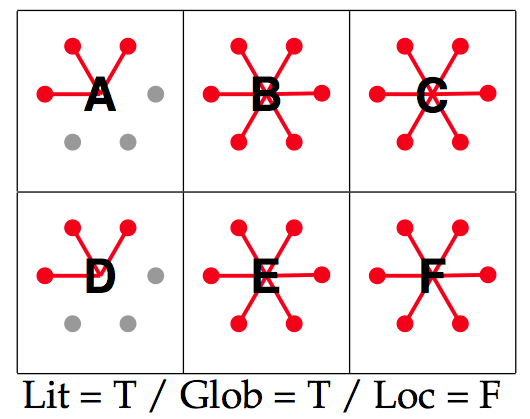
\includegraphics[scale=0.35]{Chemla_Spector_2010_Critical_AE.png}\\
      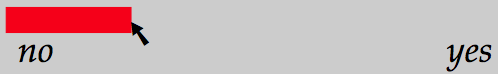
\includegraphics[scale=0.35]{Chemla_Spector_2010_RatingBar.png}
        \caption{Example of critical trial for \as-condition by
          \citeauthor{ChemlaSpector2010:Experimental-Ev}'s
          (\citeyear{ChemlaSpector2010:Experimental-Ev})}
  \label{fig:Chemla-Spector}
\end{figure}

Albeit in a different format, the pictures used by
\citeauthor{ChemlaSpector2010:Experimental-Ev} were all different
instantiation of the situation types in
Figures~\ref{fig:AS-distinguishing-pics} and
\ref{fig:ES-distinguishing-pics}. The results reported in this study
are averaged clicking positions, as shown in
Figure~\ref{fig:Chemla-Spector-Results}.
%
\begin{figure}
  \centering
  \subfloat[][\as-condition]{
    \label{fig:CS-Results-as}
        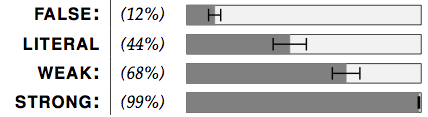
\includegraphics[width=5.5cm]{Chemla_Spector_2010_Results_AE.png}
  }
  \subfloat[test][\es-condition]{
    \label{fig:CS-Results-es}
    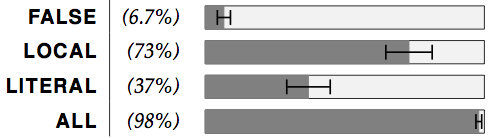
\includegraphics[width=5.5cm]{Chemla_Spector_2010_Results_GE.png}
  }
  \caption{Results from
    \citeauthor{ChemlaSpector2010:Experimental-Ev}'s
    (\citeyear{ChemlaSpector2010:Experimental-Ev}) study}
  \label{fig:Chemla-Spector-Results}
\end{figure}
%
According to \citeauthor{ChemlaSpector2010:Experimental-Ev}, the
crucial piece of evidence for the availability of local readings for
\as-sentences was that these sentences yielded higher graded
acceptability scores for the strong situation than for the weak
situation (although these differ only with respect to the truth value
of the local reading). In a similar way, evidence for the availability
of the local reading for \es-sentences comes from the difference
between the local and the literal situation. Strikingly, in the latter
case, the \es-sentences received an average of 73\% acceptability in
the local situation although the literal and global readings are false
in this case.


\subsection{Critique}
\label{sec:critique}

Summing up, the mentioned studies have presented diverging evidence
concerning the availability of local readings. Varoius problematic
aspects of these studies have already been discussed elsewhere
\citep[e.g.][]{CliftonDube2010:Embedded-Implic,ChemlaSpector2010:Experimental-Ev,Tielvan-Tiel2012:Embedded-Scalar}. Here,
we want to point out two particular methodological problems that do
impede their interpretation. However, we also want to make clear that
these problems follow almost directly from the nature of the
phenomenon under investigation and therefore seem nearly impossible to
avoid.

Firstly, a mapping between responses in a picture-verification task
and readings of the relevant sentences is problematic due to the
logical dependencies between the relevant readings discussed in
Section~\ref{sec:get-know-your}. Let us consider \as-sentences in the
following because these have been addressed by all three
aforementioned studies. (Similar arguments apply to \es-sentences.) It
is impossible to construct situations that clearly correspond to local
readings of \as-sentences, since the local reading of such sentences
implies their global and local readings. Every situation which is
consistent with such a sentence under its local reading is also
consistent with the other two readings. Therefore, we cannot test
directly and independently all the cases we might wish to using a
simple picture-verification paradigm. It would be especially desirable
to test situations that are consistent with the local reading, but
inconsistent with the global and literal reading. In that case
\emph{yes}-responses would unambiguously indicate availability of
local readings. However, since this is impossible we are left with
suboptimal choices. In the experiment of
\citet{GeurtsPouscoulous2009:Embedded-Implic} situations that are
inconsistent with local readings but consistent with the other two
readings were tested. In that case \emph{no}-responses would be decisive~--
when compared to a suitable baseline. However, \emph{yes}-responses were
observed exclusively. These can be attributed to one of the other
readings. Therefore, assuming a principle of charity
\citep{Davidson1973:Radical-Interpr} to be at play in picture
verification tasks, the data of Geurts do not provide evidence against
the existence of local readings.  In the experiments of C\&S and C\&D
on the other hand situations that are consistent with all three
readings were tested. Here again 'yes'-judgments cannot be interpreted
confidently because they can always be attributed to global or literal
readings. Both C\&S and C\&D attempt to surpass this problem by
interpreting relative preferences. This does, however, bring us to the
second problem.

Preferences may be affectd by graphical properties of the picture
materials. For example, verification complexity or typicality of the
pictures with respect to the test sentences may differ between
conditions and thereby induce certain preferences. In his careful
critique van Tiel has eleborated on this point. Van Tiel points out
that the relative preferences C\&S and C\&D interpret can be explained
solely in terms of typicality, because the `strong'-situation (see
e.g.~Figure~\ref{fig:strong}) are more typical instances of the
sentence meaning than the competing pictures, irrespective of local
implicatures.

To conclude, in order to decide about the availablity of local
implicatures we would ideally like to test situations that can
unambiguously be mapped to the different readings and do not differ in
typcality or other crucial properties. Given the logical dependencies
inherent to the relevant readings and the considerations concerning
typicality presented by van Tiel this seems impossible to achieve. As
we willl argue below we do, however, believe it is.

\subsection{To-Be-Included Here}
\label{sec:whats-missing}

\begin{itemize}
\item establish independence (as much as possible) of pictorial
  complexity/stereotypicality and assessment of reading
  \begin{itemize}
  \item not desirable to raise the level of relevance of local
    readings, because we want to test the base-line / default (cite
    Geurts / van Tiel)
  \item unclear what graded truth-value judgements measure exactly
    (re-read \citet{Chemla2009:Presuppositions} if needed)
  \item cannot separate judgements about sentences from judgements
    about pictures (van Tiel)
  \item unclear whether design assesses preferences of readings or
    targets pictorial complexity / typicality (van Tiel)
  \end{itemize}
\item provide a benchmark from which to deduce preference relations
\item control for intonational pattern (present auditorily)
  \begin{itemize}
  \item intonational effects discussed by
    \citet{Horn2006:The-Border-Wars,Geurts2009:Scalar-Implicat,Geurts2010:Quantity-Implic},
    \citep[c.f.][]{ChemlaSpector2010:Experimental-Ev}
  \item mention \citet{SchwarzClifton2008:Strengthening-o} (re-read,
    check for newer version)
  \end{itemize}
\item different languages
\end{itemize}





\section{An Incremental Verification Task}
\label{sec:exp}

\subsection{Design}
\label{sec:design}

\paragraph{General Idea.} In order to test whether local readings
are available, we seeked for a way to unambiguously map responses from
a picture verification task to the alternative readings of \as- and
\es-sentences. In addition, we wanted to minimize effects of any
graphical differences between the picture materials. To achieve this
we designed an experiment employing a modified version of picture
verification, namely the incremental verification task (IVT, see
Conroy). We will now describe the design step by step.

Consider the \as-sentence in (\ref{ex:as}). With respect to figure
\ref{fig:exseqAS3} the local reading is false, while the global and
literal reading is true. Now, we made use of the following fact. If we
cover up certain edges in the graph as in Figure \ref{fig:exseqAS2}
the literal and global reading is still true, but the local reading is
not decidable (assuming we haven't seen the whole graph, yet). By
covering even a greater part of the graph, we can go one step
further. In Figure \ref{fig:exseqAS1} the literal reading is true,
while the local and global reading cannot be decided, yet. Now,
consider the following task. Participants are asked to read sentence
(\ref{ex:as}) and then uncover a graph step by step until they feel
able to give a truth value judgment. In this task the participant has
three options at each step: (1) demand more information (2) judge the
sentence as true (3) judge the sentence as false. Presenting a
sequence like Figure \ref{fig:exseqAS}, we obtain the desired mapping
between judgments and readings. This mapping is illustrated in Figure
\ref{fig:mappingAS}.


For the \es-sentences, the idea is similar. With respect to the
sentence in (\ref{ex:es}) we obtain an unambiguous mapping between
truth values and readings with respect to the sequence in
\ref{fig:exseqES}. This is illustrated in Figure
\ref{fig:mappingES}. There are two differences to the previous
case. Firstly, the order of readings that can be identified in the
sequence differs. At the first step the global reading can be
judged. Then the literal and, finally, the local reading can be
judged. Secondly, the readings correspond to different truth
values. Global and literal readings correspond to negative truth
values, while local reading require positive judgments.

\begin{exe}
\ex \gll \mymark{Jeder} Brief ist mit \mymark{einigen} seiner Dreiecke
  verbunden.\dn{these are not the sentences we used, right?}  \label{ex:as}\\
Every Letter is with some its triangles connected.\\
\trans Every letter is connected to some of its triangles.
\end{exe}


\begin{exe}
\ex \label{ex:es} \gll \mymark{Genau} eine Glocke ist mit \mymark{einigen} ihrer Halbkreise verbunden.\\
  Exactly one Letter is with some its semicircles connected.\\
  \trans Exactly one letter is connected to some of its semicircless.
\end{exe}


\begin{figure}[ht]
	\centering
	\subfloat[][Step 3]{ 
		\fbox{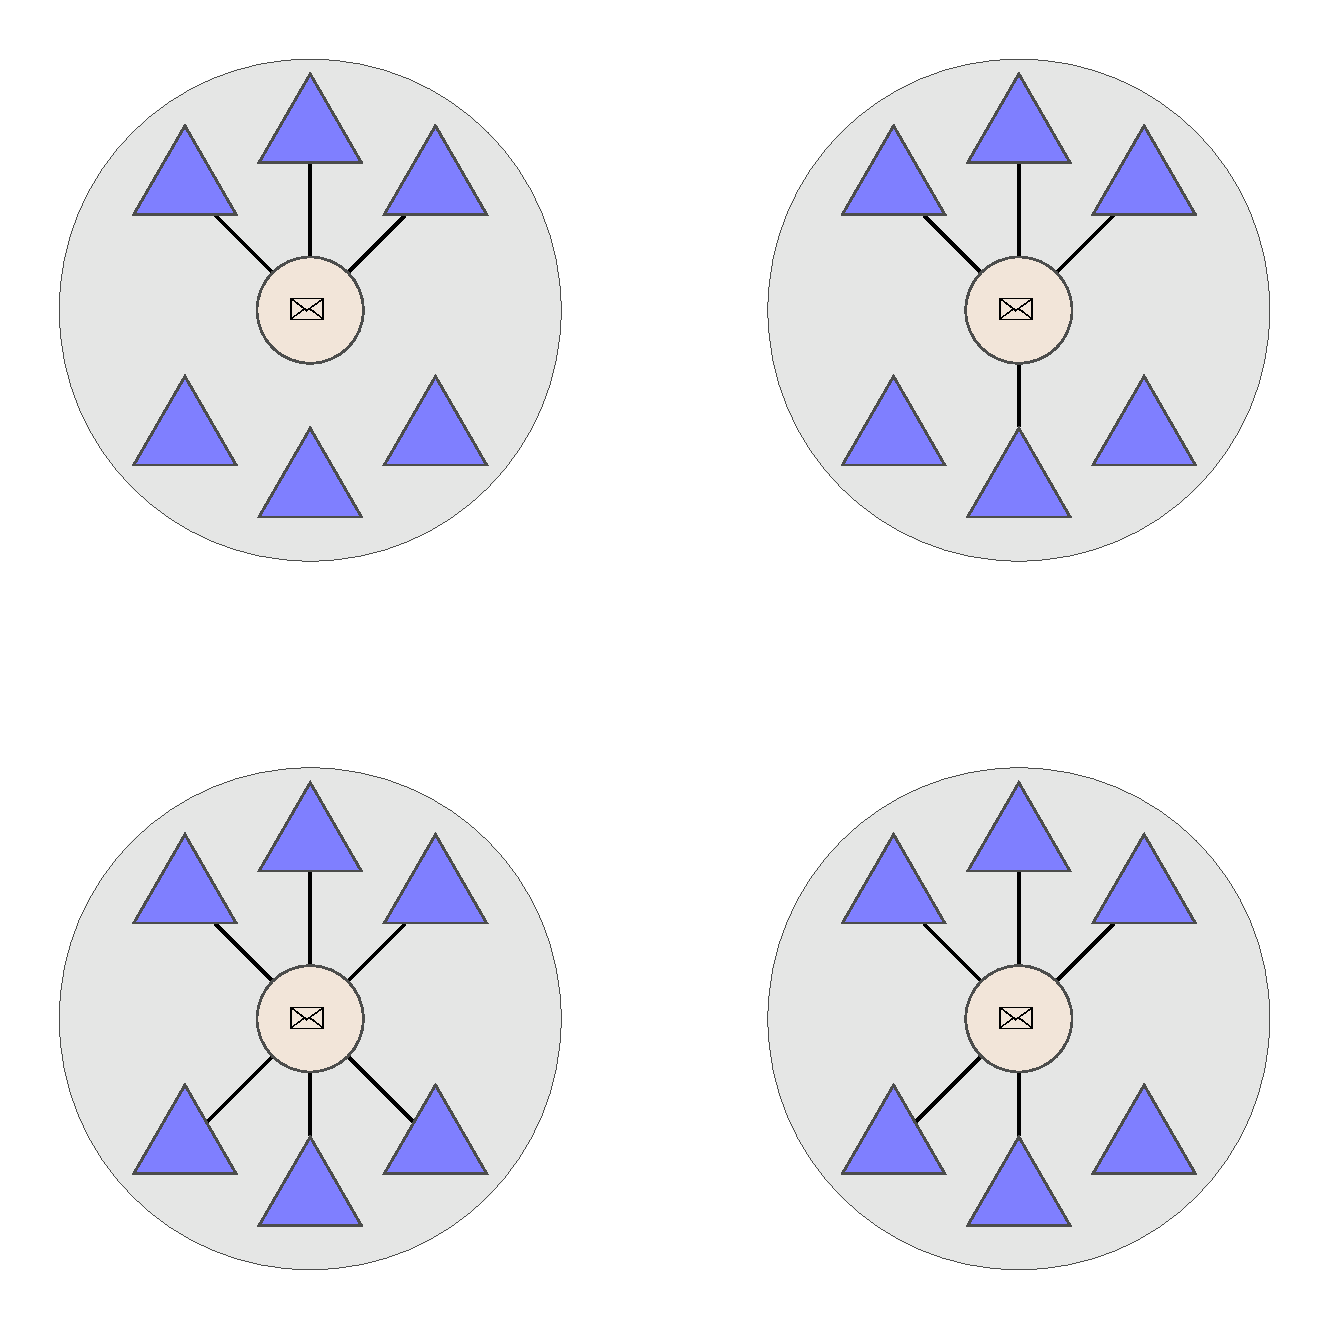
\includegraphics[width=3cm]{../pictures/paper/ae_7_v_l.pdf}}
	    \label{fig:exseqAS3}
	}
	\subfloat[][Step 2]{
		\fbox{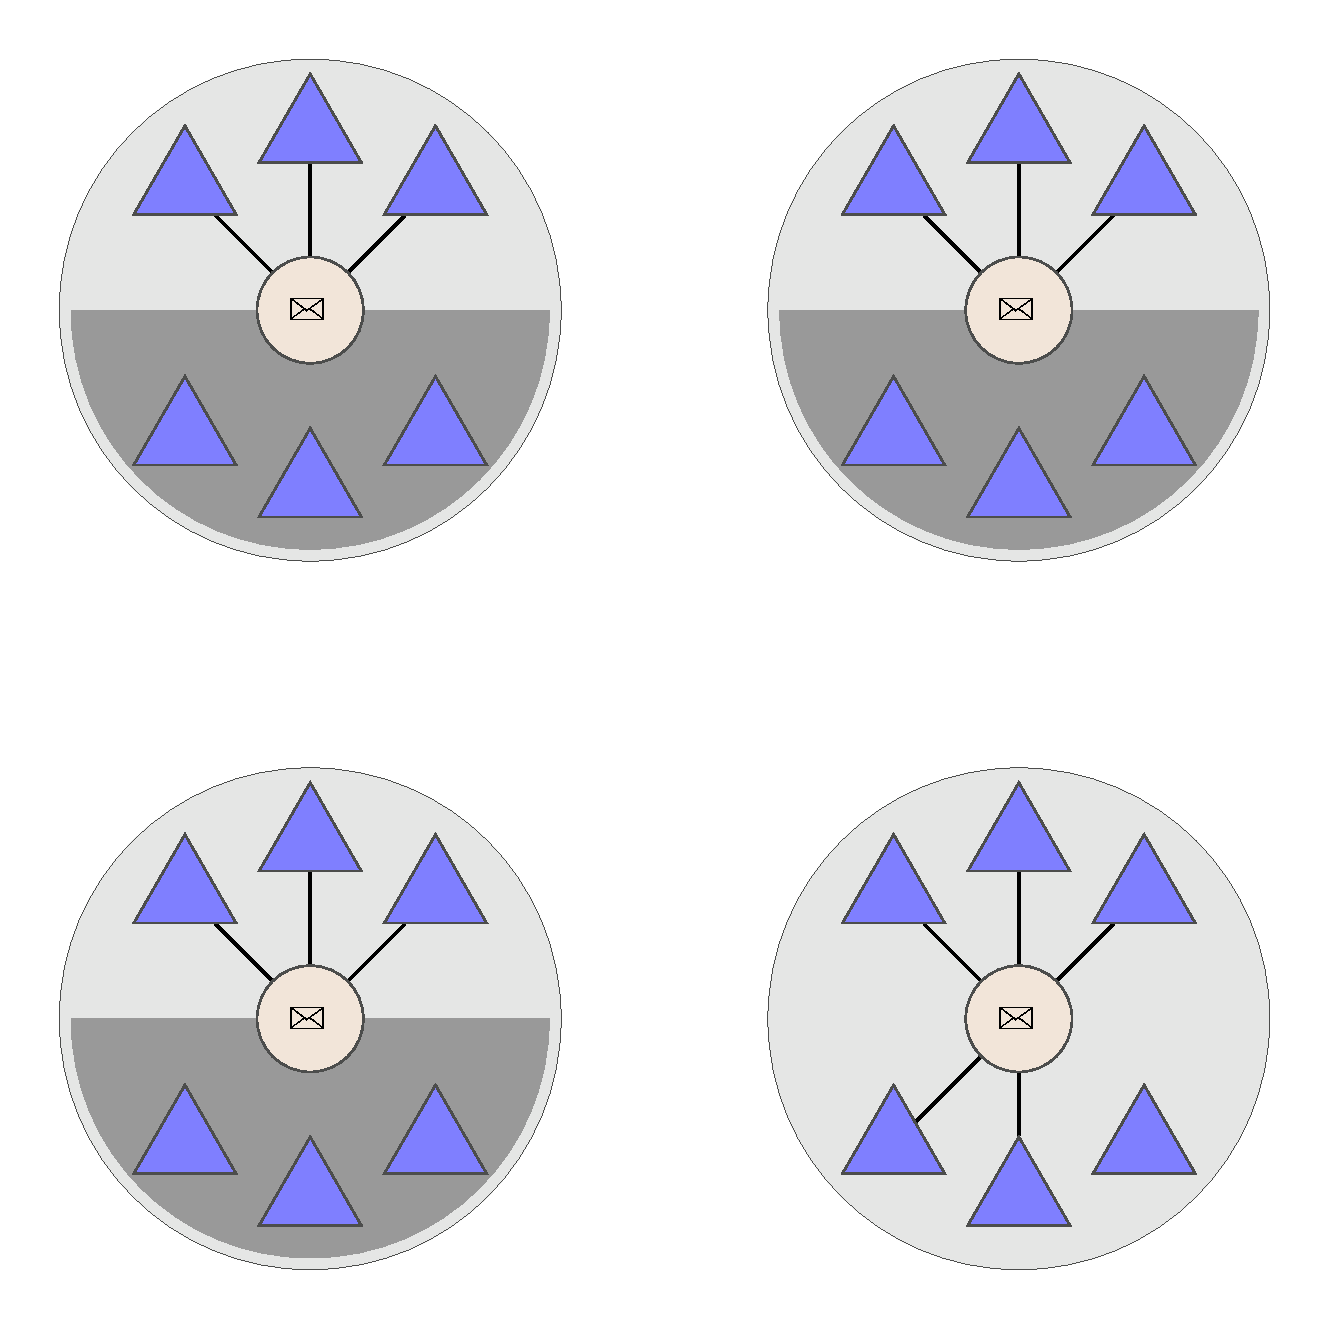
\includegraphics[width=3cm]{../pictures/paper/ae_5_v_l.pdf}}
	    \label{fig:exseqAS2}
	}
	\subfloat[][Step 1]{ 
		\fbox{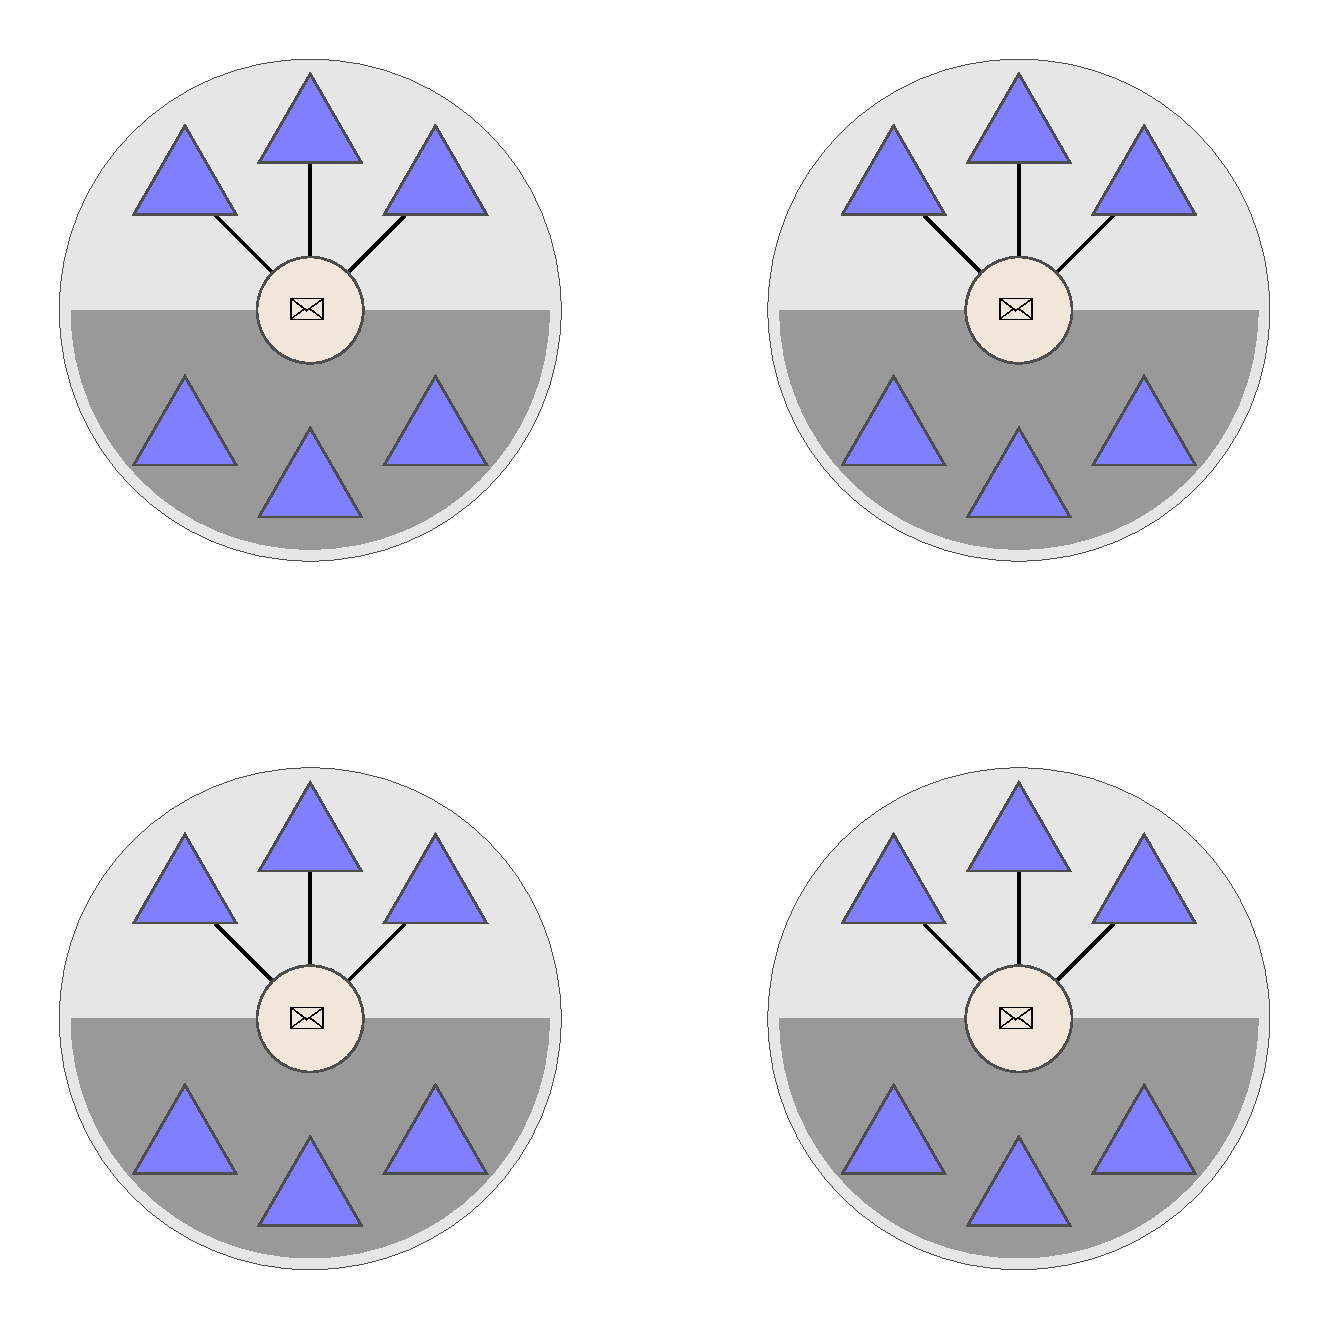
\includegraphics[width=3cm]{../pictures/paper/ae_3_v_l.pdf}}
	    \label{fig:exseqAS1}
	}
	\caption[]{Example sequence for \as-sentences}
	\label{fig:exseqAS}
\end{figure}

\begin{figure}[ht]
	\centering
	\subfloat[][Step 3]{ 
		\fbox{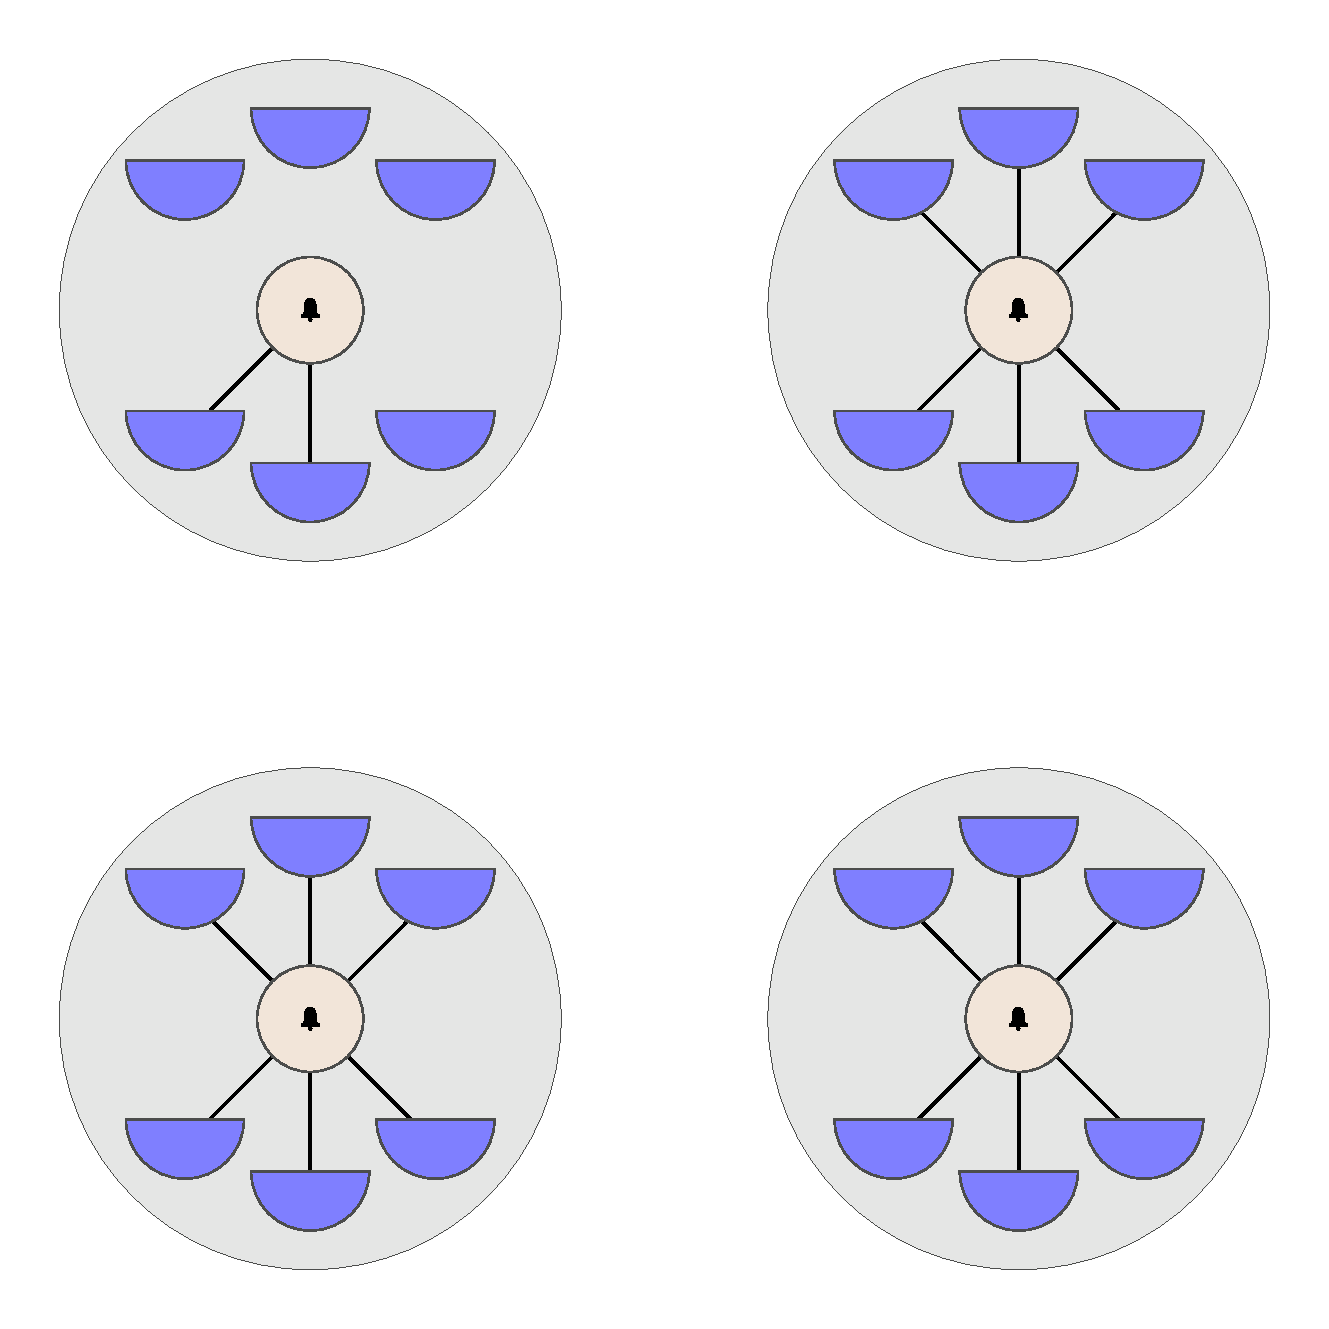
\includegraphics[width=3cm]{../pictures/paper/ge_6_v_l.pdf}}
	    \label{fig:subfig1}
	}
	\subfloat[][Step 2]{
		\fbox{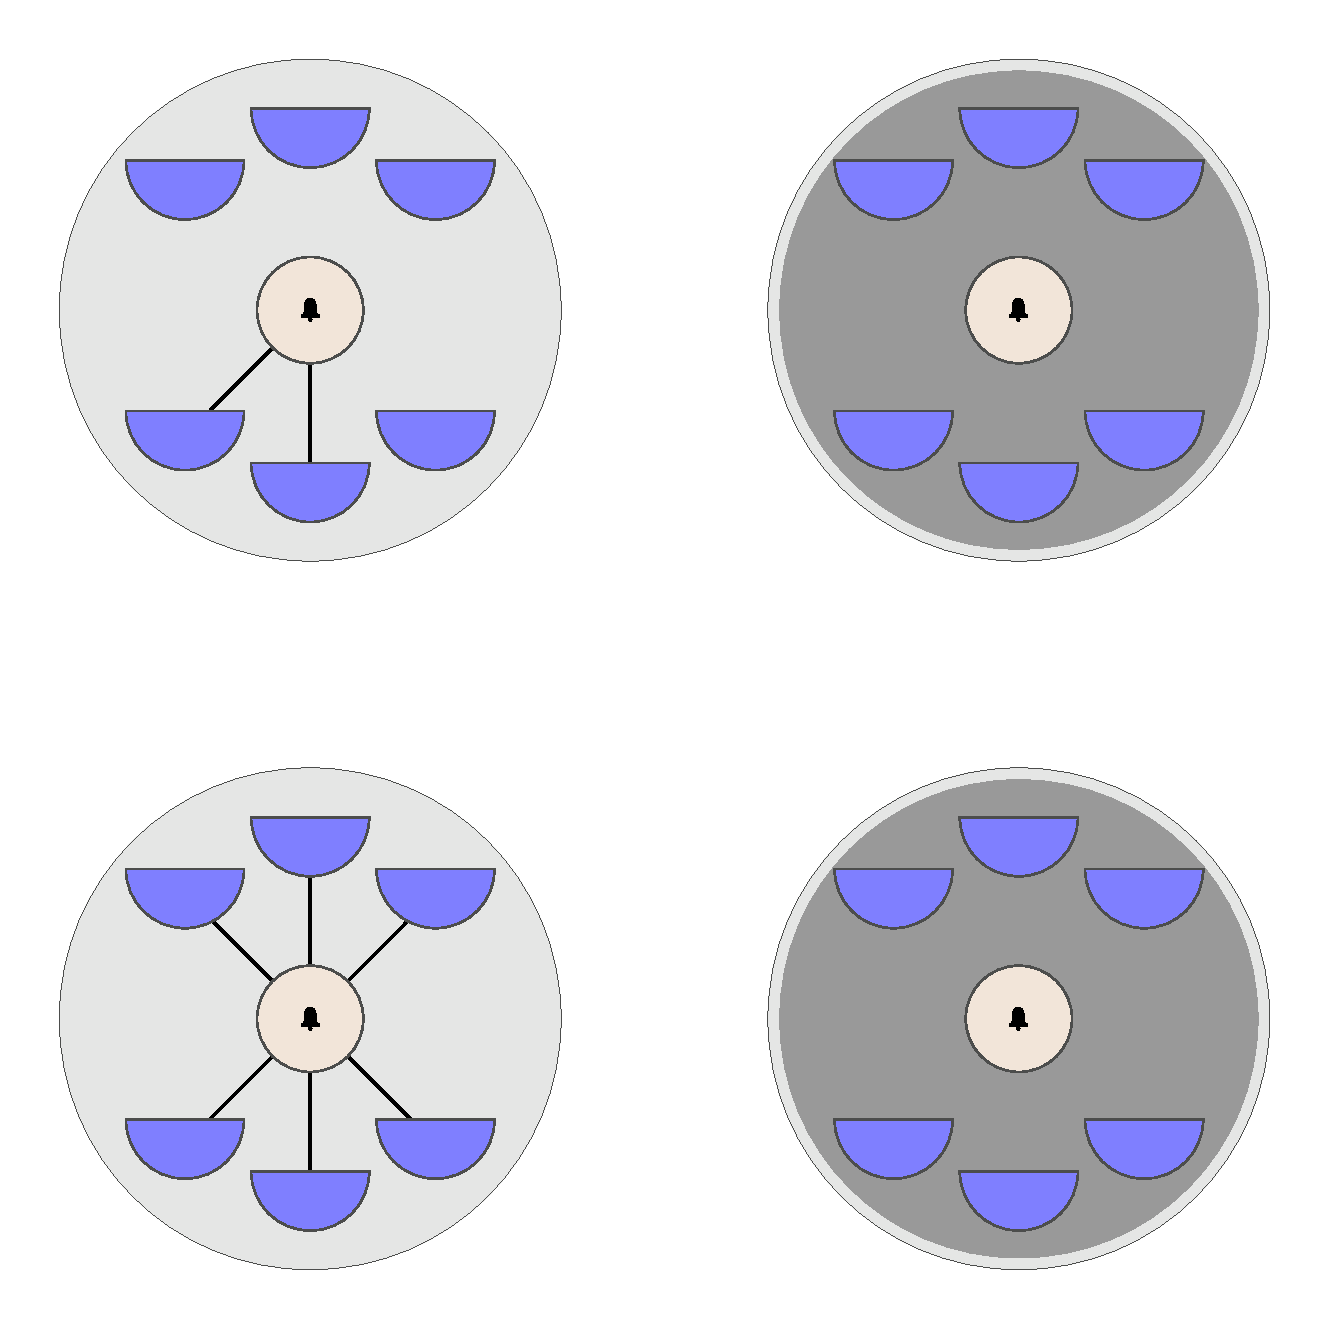
\includegraphics[width=3cm]{../pictures/paper/ge_4_v_l.pdf}}
	    \label{fig:subfig2}
	}
	\subfloat[][Step 1]{ 
		\fbox{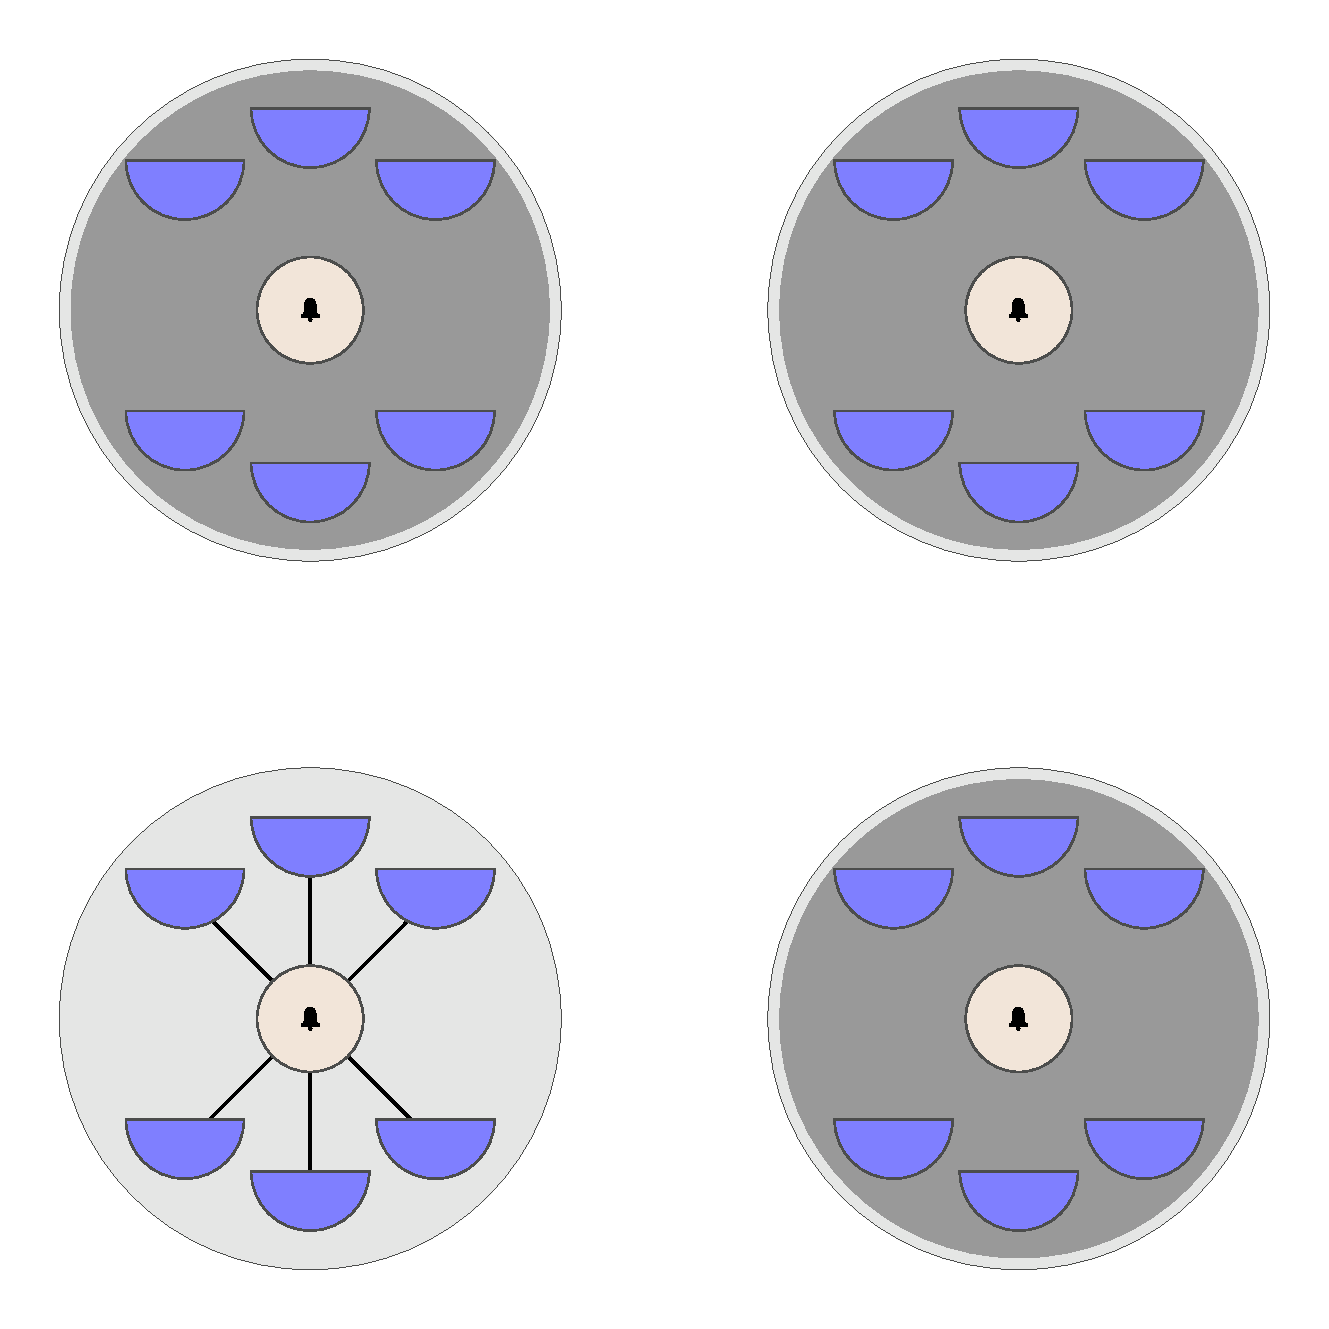
\includegraphics[width=3cm]{../pictures/paper/ge_3_v_l.pdf}}
	    \label{fig:subfig1}
	}
	\caption[]{Example sequence for \as-sentences}
	\label{fig:exseqES}
\end{figure}






\begin{figure}[ht]
	\centering
	\subfloat[][\as-Sentences]{ 
\begin{tabular}{cccc}
&more info&true&false\\
\hline
Step 1&?&literal&?\\
Step 2&?&global&?\\
Step 3&?&?&local\\
\hline
\end{tabular}

	    \label{fig:mappingAS}
	}
	\subfloat[][\es-Sentences]{
\begin{tabular}{cccc}
&more info&true&false\\
\hline
Step 1&?&literal&?\\
Step 2&?&global&?\\
Step 3&?&?&local\\
\hline
\end{tabular}
	    \label{fig:mappingES}
	}
\caption{Mapping from truth values to readings}
\label{fig:subfigureExample}
\end{figure}


In addition to the unambiguous mapping from readings to truth values,
we think that the present design minimizes graphical effects because
there is no comparison between different pictures. The distribution of
responses found in previous studies could in part be explained by
differences in typicality of the pictures with respect to the possible
readings (see van Tiel). In the present case this kind of reasoning
would have to be extended to the typicalilty of parts of pictures. On
intuitive grounds, we take this kind of reasoning to be
implausible. We will now shortly discuss how graphical properties
might still affect judgments in the worst case. In the first step of
the \as-condition local and global readings cannot be judged,
yet. Therefore, graphical properties should not affect judgments if
participants have one of these readings in mind. If participants have
a literal reading in mind, the worst case scenario is that they
refrain from judging the sentence as true at this point due to some,
eg. atypical, graphical property of the picture. The situation is
similar at the second step. The local reading is still not
decidable. Therefore, graphical properties should not play a role if
participants have a local reading in mind. A positive judgment might,
however, be a delayed judgment of a literal reading. Again, the worst
case scenario for our purpose is that participants refrain from
answering because of graphical properties. At the last step the local
reading requires a negative judgment. Now, we could obtain delayed
negative responses from literal or global readings because the graph
as a whole is, e.g., logically true but atypical with respect to these
readings. These kinds of judgments would be indistinguishable from
local responses. Note, however, that we have no reason to believe that
typicality has large effects, because, given the results from van
Tiel, the picture as a whole is expected to be one of the more typical
situations for \as-sentences. Still, we cannot exclude the possibility
that graphical properties of the pictures might have the described
effect. In the \es-conditions this type of effect is, however, entirely
impossible since the literal and global reading is plainly false given
the initial parts as well as the whole graph. Summing up, in the worst
case, which we consider implausible, graphical effects might lead to
an enhanced number of local responses in the \as- as compared to the
\es-condition. We have to keep this possibility in mind. We want to
stress, however, that the design presented here improves on previous
studies with respect to possible graphical effects.

\paragraph{Testing Effects of accentuation.} It has been claimed that
local readings only emerge in the case of special accentuation of the
the scalar item under consideration (REFERENCES). Further, it is
generally assumed that the required type of accentuation is a pitch
accent (REFS). To test for this possibility we decided to present the
sentences (eg., (\ref{ex:as}) and (\ref{ex:es})) auditively in two
versions each. In the accented version a pitch accent was palced on
{\it einige}. The second version had neutral prosody. If accentuation
is the driving force for local readings, we would expect a higher
proportion of local readings in the former than in the latter version
of the sentences.

\paragraph{Controlling Response biases.} In order to control for
response biases that are independent of the sentence meaning, but only
depend on the experimental procedure or on the picture materials, we
generated a set of control conditions. For all three readings in the
\as- and \es-conditions we constructed one unambiguous control sentence
requiring the same type of response at the same point in the
sequence. We used sentences as in (\ref{bsp:controls-as}) and
(\ref{bsp:controls-es}). Example (\ref{bsp:controls-as-1}) requires
the same response as the \as-sentence in \ref{ex:as} under its literal
reading, (\ref{bsp:controls-as-2}) corresponds to the \as-sentence
under its global reading and (\ref{bsp:controls-as-3}) corresponds to
the local reading. With regard to the \es-sentences, controls like
(\ref{bsp:controls-es-1}) correspond to the global reading,
(\ref{bsp:controls-es-2}) to the literal and
(\ref{bsp:controls-es-3}) to the local reading.  If, independently
from sentence meaning, there was any bias to respond in a certain way
at any point in the sequences this should affect the control sentences
to the same degree as it affects the target conditions.

\begin{exe}
  \ex \label{bsp:controls-as}
    \begin{xlist}
\ex \label{bsp:controls-as-1} \gll Alle W\"urfel sind mit mindestens drei ihrer Dreiecke verbunden.\\
  All dice are with at-least three their triangles connected.\\
  \trans All dice are connected to at least three of their triangles.
\ex \label{bsp:controls-as-2} \gll Mindestens ein Brief ist mit genau f\"unf seiner Quadrate verbunden.\\
  At-least one letter is with exactly five his squares connected.\\
  \trans At least one letter is connected with exactly five of his squares.
\ex \label{bsp:controls-as-3} \gll Jeder Brief ist mit mindestens vier seiner Quadrate verbunden.\\
  Every letter is with at-least four his squares connected.\\
  \trans Every letter is connected to at least four of its squares.
\end{xlist}

\end{exe}



\begin{exe}
\ex \label{bsp:controls-es}
  \begin{xlist}
\ex \label{bsp:controls-es-1} \gll Alle Glocken sind mit weniger als vier ihrer Halbkreise verbunden. \\
All bells are with fewer than four their semicircles connected.\\
\trans All bells are connected with fewer than four of their semicircles.  
\ex \label{bsp:controls-es-2} \gll Alle Glocken sind mit allen ihren Halbkreisen verbunden.\\
All bells are with all their semicircles connected.\\
\trans All bells are connected to all of their semicircles. 
\ex \label{bsp:controls-es-3} \gll Mindestens drei Glocken sind mit allen ihren Halbkreisen verbunden.\\
  At-least three bells are with all  their semicircles connected.\\
  \trans At least three bells are connectd with all of their semicircles.
\end{xlist}

\end{exe}




\paragraph{Controlling ambiguity resolution.} In order to confidently
interpret the results obtained in the described IVT experiment, we
need to know certain facts about how participants deal with ambiguous
sentences in the IVT (disccussion of Conroy's study). To investigate
this we used a second type of control conditions. In particular, we
tested (1) whether the order in which readings can be judged affects
preferences for ambiguous sentences and (2) whether prosodic
information can, in principle, shift reading preferences in the
present task. To this end, we used ambiguous sentences of the type in
(\ref{bsp:target-related}). In the literature (REFS) two readings are
reported for sentences of this kind. Under the first reading the PP
{\it with suns} modifies the complete conjunction {\it circles and
  squares}. This reading is called the high-attachment reading. Under
the second, low-attachment, reading the PP only modifies the second
conjunct, {\it squares}. Generally, the late closure reading is
preferred over the early closure reading for sentences like
(\ref{bsp:target-related}) (REFS). Concerning presentation order of
readings, it is crucial for our purpose that dispreferd readings are
in principle detectable regardless of their position in the
sequence. To test this we combined sentences like
(\ref{bsp:target-related}) with two kinds of sequences. In the first
kind of sequence a partly uncovered graph like in figure
\ref{fig:exec1} preceeds a graph like in figure \ref{fig:exec2}. Here,
the high-attachment reading can be judged first. Under this reading we
would expect a "no"-judgment on \ref{fig:exec1}. Under the
low-attachment reading we would, in contrast, expect a "yes"-response
on \ref{fig:exec2}. The order of presentation is reversed in the
second kind of sequence which included pictures like \ref{fig:exlc1}
folllowed by pictures like \ref{fig:exlc2}. Here, the low-attachment
reading can be judged first requiring a "yes"-response on
\ref{fig:exlc1}. The high-attachment reading can only be judged later
in the sequence. When we reach \ref{fig:exlc2} a "no"-response is
expected under a high-attachment reading. If presentation order does
affect preferences, we would expect preferences to differ between the
two types of sequences.

\begin{exe}
\ex \gll Der Brief ist mit Kreisen und Vierecken mit Sonnen
  verbunden. \label{bsp:target-related}\\
The letter is with circles and squares with suns connected.\\
The letter is connected with circles and squares with suns.
\end{exe}


\begin{figure}[ht]
	\centering
	\subfloat[][Step 1]{ 
		\fbox{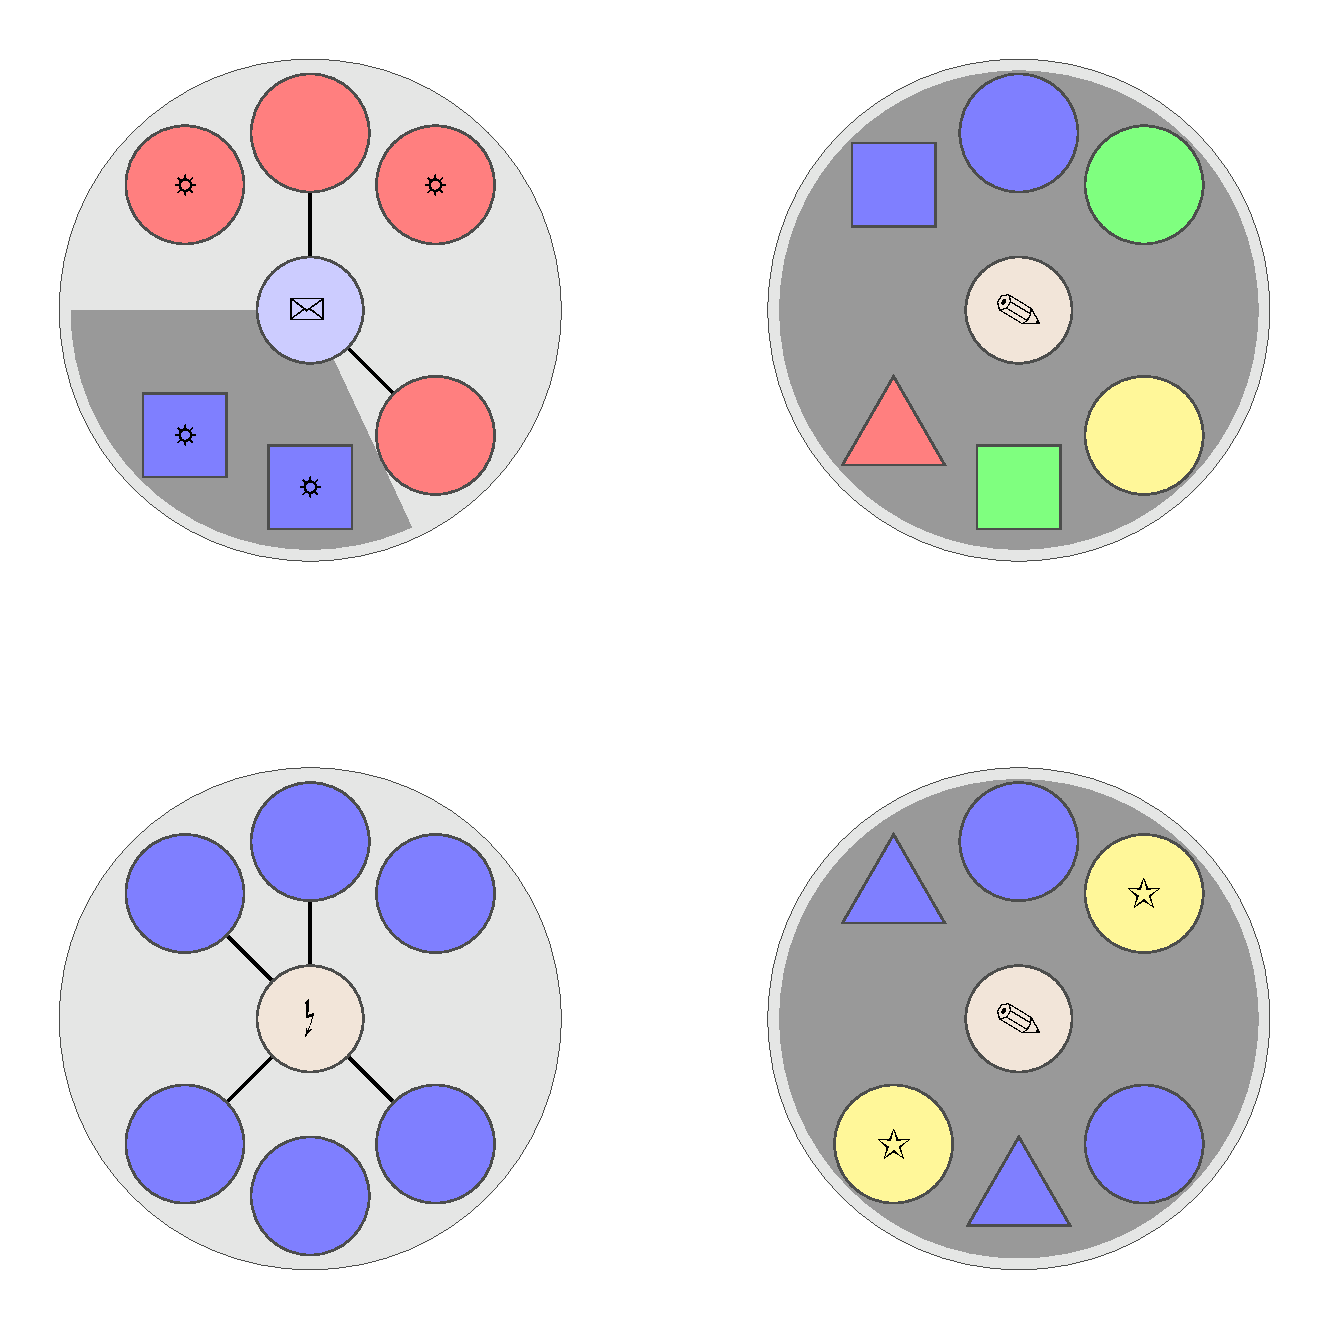
\includegraphics[width=3cm]{../pictures/paper/ec_01_3.pdf}}
	    \label{fig:exec1}
	}
	\subfloat[][Step 2]{
		\fbox{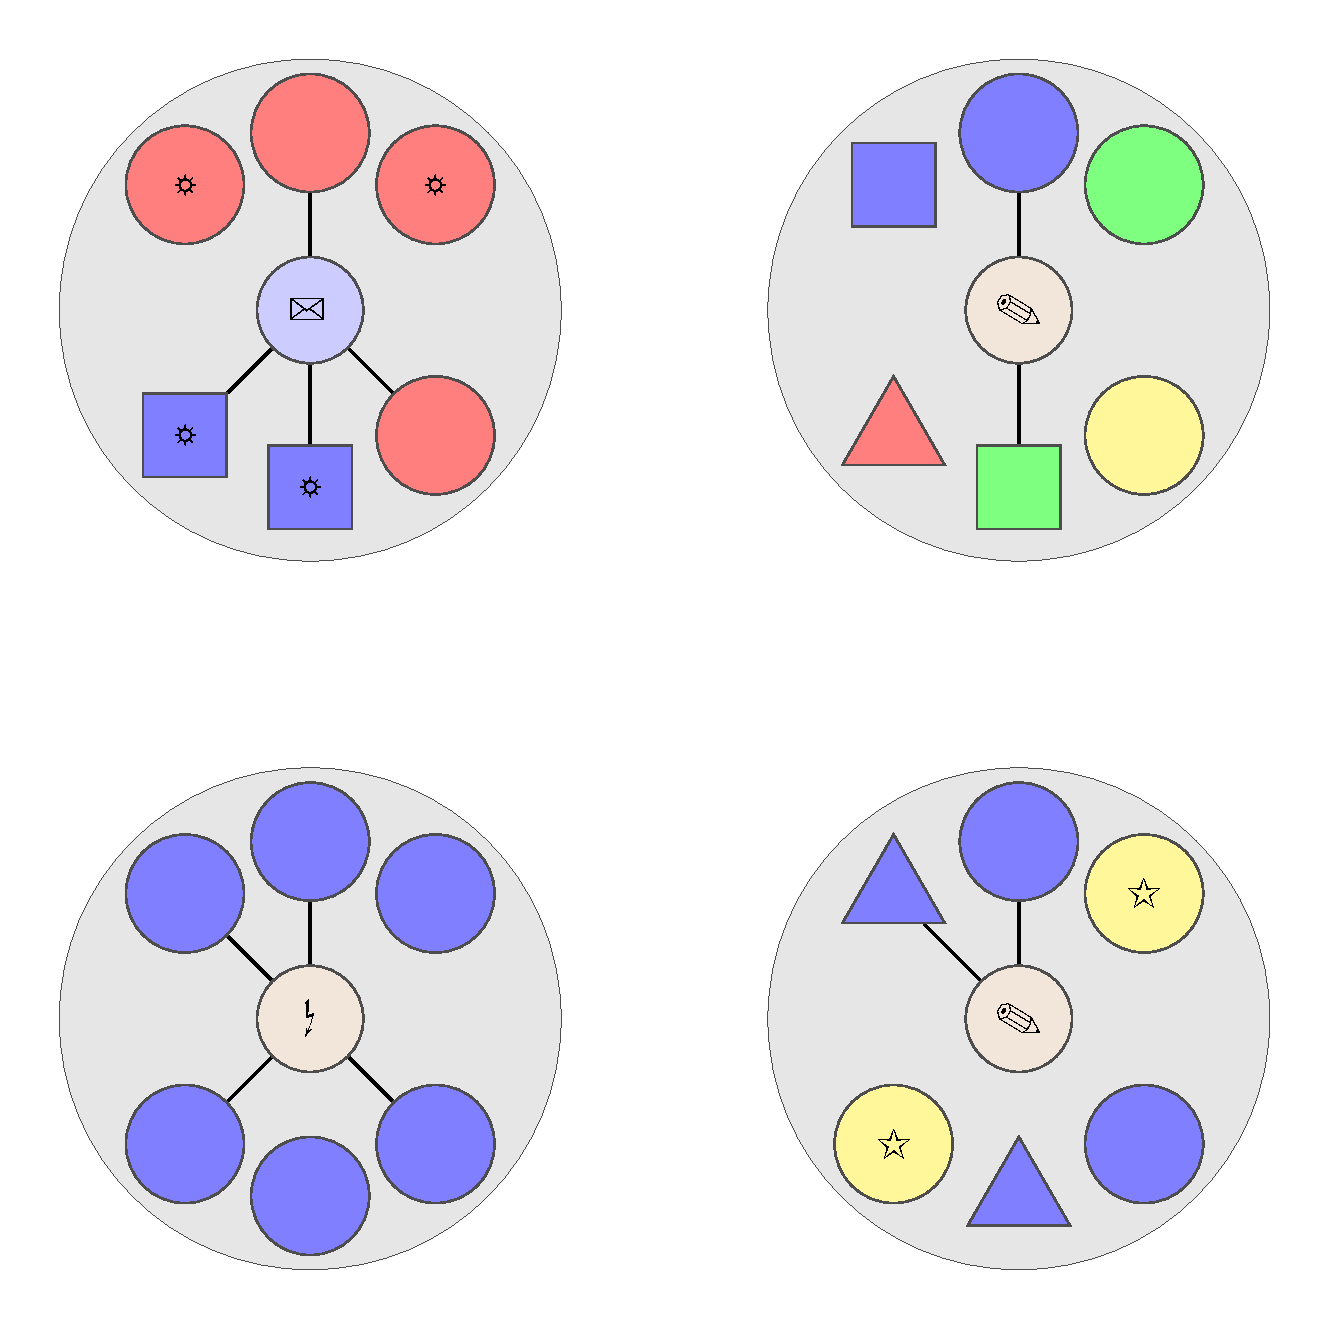
\includegraphics[width=3cm]{../pictures/paper/ec_01_5.pdf}}
	    \label{fig:exec2}
	}
	\caption[]{High-attachment first}
	\label{fig:exec}
\end{figure}

\begin{figure}[ht]
	\centering
	\subfloat[][Step 1]{ 
		\fbox{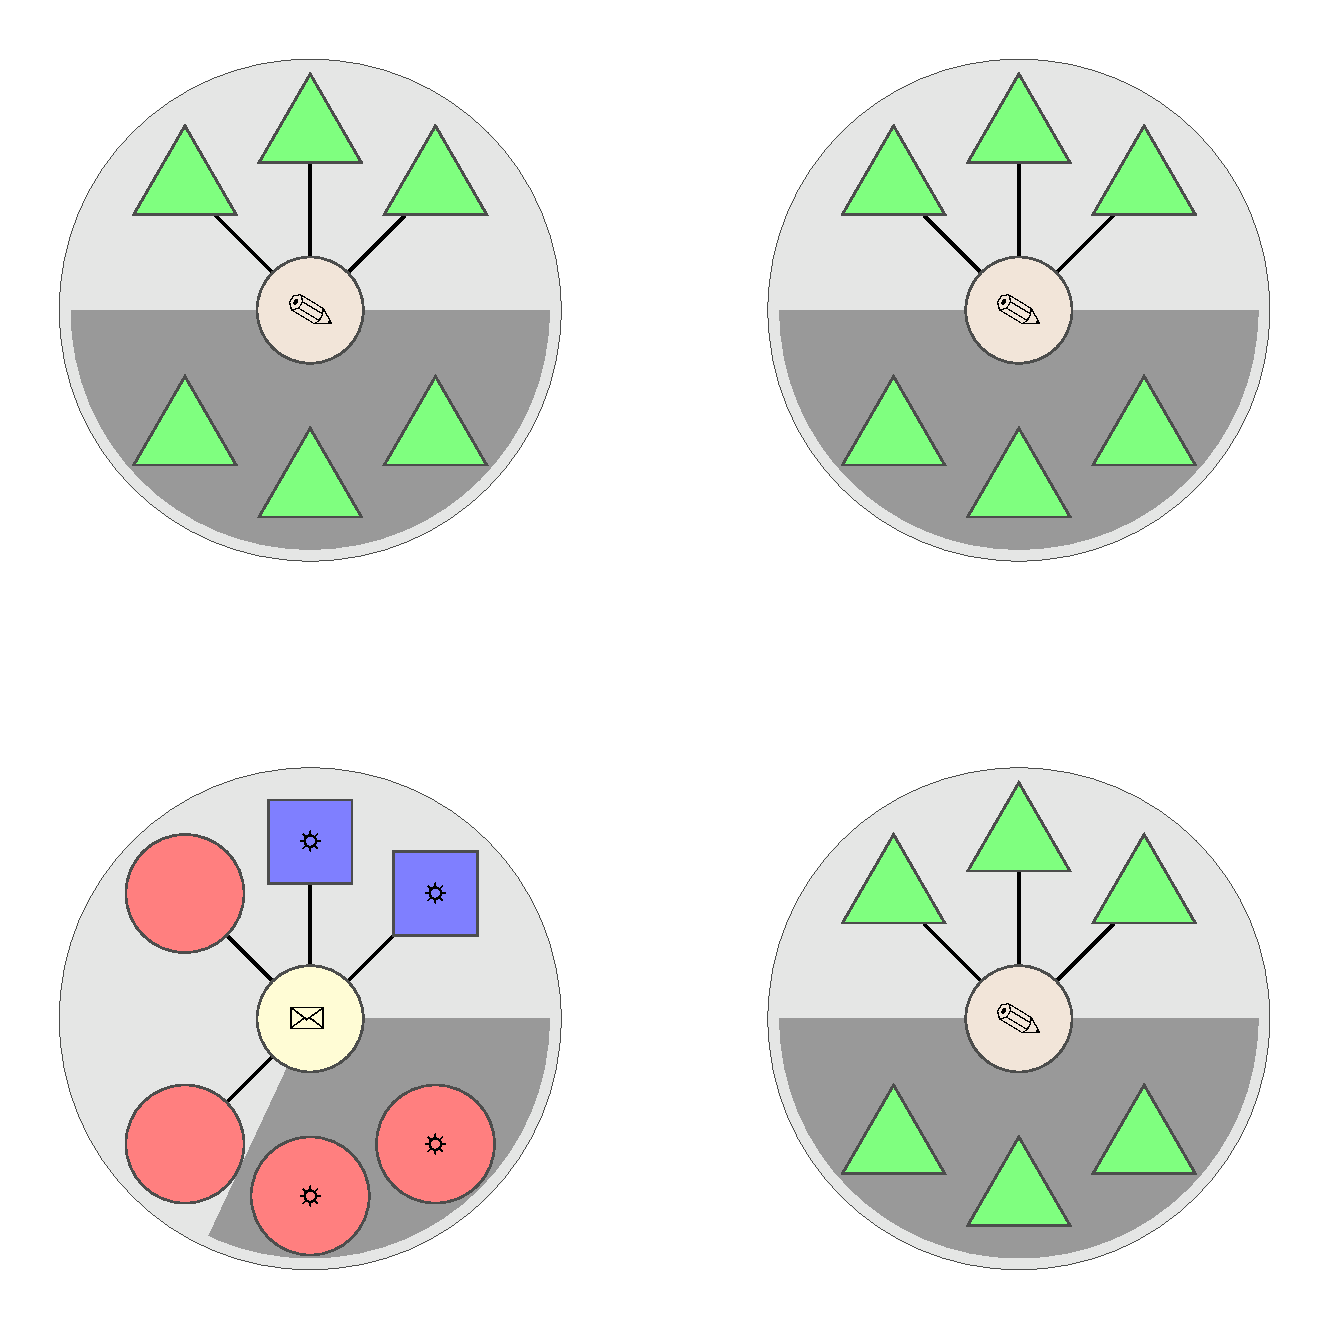
\includegraphics[width=3cm]{../pictures/paper/lc_01_3.pdf}}
	    \label{fig:exlc1}
	}
	\subfloat[][Step 2]{
		\fbox{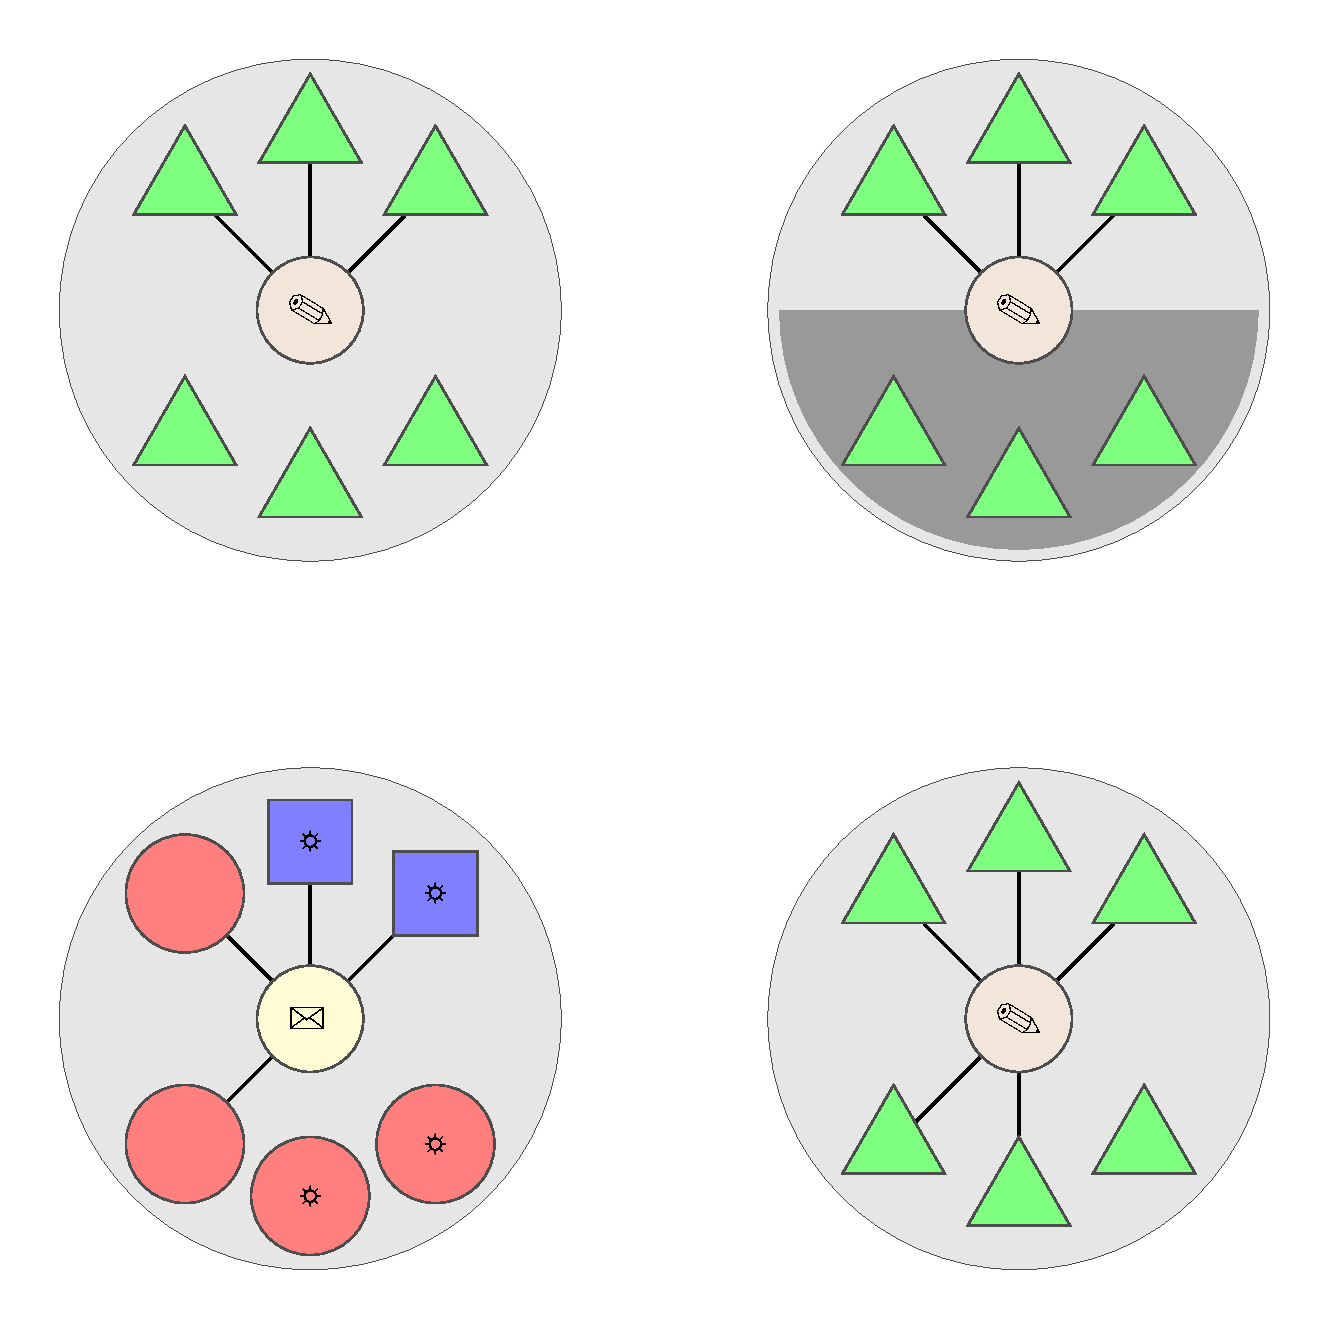
\includegraphics[width=3cm]{../pictures/paper/lc_01_6.pdf}}
	    \label{fig:exlc2}
	}
	\caption[]{Low-attachment first}
	\label{fig:exec}
\end{figure}

Concerning prosodic information, we wanted to make sure that
differences in prosody may generally lead to a shift in interpretation
preferences in the ITV task. Sentences like (\ref{bsp:target-related})
are well suited to test this assumption since it is well-known that
their interpretational preferences are sensitive to prosody. The most
natural way to pronounce a sentence like (\ref{bsp:target-related})
includes a prosodic phrase boundary between {\it squares} and {\it
  with}. This intonation pattern strongly corresponds to the
high-attachment reading. If, instead, a prosodic phrase boundary after
{\it circles} is present, the acceptance of the low-attachment reading
is boosted. To test whether prosodic information is taken into account
in the IVT we presented both types of prosodic structures expecting
the described boost in acceptance for the low-attachment reading. In
addition, we also included a neutral version containing no phrase
marking whatsoever. This should receive intermediate acceptance
rates. Further, we also presented unambiguous sentences corresponding
to the early closure reading. As in the case of the \as- and
\es-sentences the unambiguous counterparts served as a baseline to
control for response biases that are independent of sentence meaning.

\subsection{Procedure}
\label{sec:procedure}   

\subsection{Materials}
\label{sec:materials}

\subsubsection{The auditory sentence material}
\label{sec:audit-sent-mater}

A phonetically trained female native speaker of German was instructed
to realize two prosodic versions of each target sentence, and four
versions of the target-related fillers. In addition to these
sentences, a set of unrelated fillers and neutral control structures
was also recorded. For these constructions, the speaker was instructed
to realize prosodic contours as neutral and natural as possible.

For all target sentences (\as and \es), the determiner \emph{some} was
produced with a contrastive pitch accent as well as with a neutral
accent, respectively. Contrastive accents in German are realized by an
H*L contour (XYZ)\dn{insert references}, thus employing a generally
falling pattern. A set of 15 experimental items was recorded for each
condition (\emph{accented} vs.~\emph{unaccented}), resulting in a
total number of 60 target sentences.

In contrast to the accent manipulation, target-related fillers
differed with respect to prosodic phrasing. Prosodic phrase boundaries
in German are realized by a rise in F0 as well as by a durational
increase on the final part of the constituent preceding the boundary
(prefinal lengthening) plus an optional pause (XYZ)\dn{references:
  Vaissiere, 1983; Fery, 1993}. Boundaries for these filler sentences
were either realized at the position separating the second \acro{pp}
from the preceding material (\emph{late boundary}, corresponding to a
high-attachment reading) or directly preceding the second conjunct in
the first \acro{pp} (\emph{early boundary}, corresponding to a
low-attachment reading). As the prosodic realization of the targets
involved the comparison between an accented and a neutral variant, we
also included a third version of target-related fillers, in which our
speaker produced the sentences without any pronounced
boundaries. Finally, an additional condition was recorded, using
disambiguated sentences that were prosodically neutral (XYZ)\dn{proper
  reference to explanation above}. For each prosodic variant, a set of
30 items was read, yielding 150 target-related fillers. Together with
30 unrelated fillers and 90 control sentences, a total number of 300
sentences was recorded. The session was recorded in an acoustically
shielded booth (44.1\,kHz sampling rate, 16 bit amplitude resolution).

Before entering the judgment task, experimental items and
target-related fillers were analyzed with respect to their acoustic
properties. As both accented elements as well as prosodic boundaries
were expected to differ with respect to their F0 and/or durational
properties, we calculated durational values as well as difference
values between minimal and maximal F0 for each word. As targets
slightly differed with respect to the total number of words as well as
with respect to certain lexical properties (i.e., \emph{seinen}
vs.~\emph{ihren}, see above (XYZ)\dn{proper reference}), we considered
the following analysis regions:

\begin{exe}
  \ex
    \begin{xlist}
      \ex $|_{\text{R}1}$~Alle  	\ $|_{\text{R}2}$~dieser 
      \ $|_{\text{R}3}$~$\acro{np}_1$  
      \ $|_{\text{R}4}$~sind  \ $|_{\text{R}5}$~mit  \
      $|_{\text{R}6}$~einigen  \ $|_{\text{R}7}$~ihrer 
       \ $|_{\text{R}8}$~{$\acro{np}_2$}  \ $|_{\text{R}9}$~verbunden.
    \ex       $|_{\text{R}1}$~Genau einer  	\ $|_{\text{R}2}$~der 
      \ $|_{\text{R}3}$~$\acro{np}_1$  
      \ $|_{\text{R}4}$~ist  \ $|_{\text{R}5}$~mit  \
      $|_{\text{R}6}$~einigen  \ $|_{\text{R}7}$~seiner 
       \ $|_{\text{R}8}$~{$\acro{np}_2$}  \ $|_{\text{R}9}$~verbunden.
    \end{xlist}
    % \begin{tabbing}
    %   $|_{\text{R}1}$ Genau einer \= 	\ $|_{\text{R}2}$ diese \=
    %   \ $|_{\text{R}3}$ \acro{np}$_1$ \= 
    %   \ $|_{\text{R}4}$ sind \= \ $|_{\text{R}5}$ mit \= \
    %   $|_{\text{R}6}$ einigen \= \ $|_{\text{R}7}$ seiner 
    %   \= \ $|_{\text{R}8}$  \acro{np}$_2$ \= \ $|_{\text{R}9}$
    %   verbunden. \kill
    %   $|_{\text{R}1}$ Alle \> 	\ $|_{\text{R}2}$ dieser \>
    %   \ $|_{\text{R}3}$ \acro{np}$_1$ \> 
    %   \ $|_{\text{R}4}$ sind \> \ $|_{\text{R}5}$ mit \> \
    %   $|_{\text{R}6}$ einigen \> \ $|_{\text{R}7}$ ihrer 
    %   \> \ $|_{\text{R}8}$  \acro{np}$_1$ \> \ $|_{\text{R}9}$
    %   verbunden. \\
    %   $|_{\text{R}1}$ Genau einer \> 	\ $|_{\text{R}2}$ der \>
    %   \ $|_{\text{R}3}$ \acro{np}$_1$ \> 
    %   \ $|_{\text{R}4}$ ist \> \ $|_{\text{R}5}$ mit \> \
    %   $|_{\text{R}6}$ einigen \> \ $|_{\text{R}7}$ seiner 
    %   \> \ $|_{\text{R}8}$  \acro{np}$_1$ \> \ $|_{\text{R}9}$ verbunden.
    % \end{tabbing}
\end{exe}

Note that differences between Regions 1, 2, 4 and 7 can be expected
due to lexical differences between the \as and \es-conditions. As
target-related fillers did not differ with respect to their lexical
properties, we carried out word-by-word analyses for these
conditions. Durational values included the respective word plus any
following silent interval. Note that we did not include the
disambiguated fillers in these analyses as they involved very
different sentence types (i.e., constructions involving prepositional
phrases vs.~relative clauses).

\begin{exe}
  \ex $|_{\text{R}1}$ \acro{D}  	\ $|_{\text{R}2}$ $\acro{np}_1$
      \ $|_{\text{R}3}$ ist 
      \ $|_{\text{R}4}$ mit  \ $|_{\text{R}5}$ $\acro{np}_2$   \
      $|_{\text{R}6}$ und  \ $|_{\text{R}7}$ $\acro{np}_3$ 
       \ $|_{\text{R}8}$  mit  \ $|_{\text{R}9}$ $\acro{np}_4$ \ $|_{\text{R}10}$~verbunden.
\end{exe}

For the durational analyses, constituents were automatically labeled
by the \emph{Aligner} tool (XYZ),\dn{reference! Rapp, 1998} and the
obtained values were manually corrected afterwards. For the targets,
two-factorial \acros{anova} with the factors \acro{Quantifier} (all
vs. exactly one) and \acro{Prosody} (accented vs.~unaccented) were
carried out. For the target-related fillers, we carried out
one-factorial \acros{anova} with the factor \acro{Prosody} (early
boundary, late boundary, neutral prosody). F0 values were extracted by
means of special Praat scripts
(\url{http://www.fon.hum.uva.nl/praat/}). For the present analyses,
differences between minimal and maximal F0 values for each region or
word were calculated. Again, two-factorial \acros{anova} were carried
out for statistical comparison of the fillers, and one-factorial
\acros{anova} were carried out for target-related structures.

\paragraph{Targets.} Table~\ref{tab:table-A} shows the durational values for each of
the single regions in the sentence. Crucially, durational values of
accented determiners were significantly increased as opposed to their
non-accented counterparts. Overall, \acro{Quantifier} effects were
observed, which might be attributed to the above-mentioned lexical
differences, as well as to the fact that \es-structures generally
contained fewer words, thus leading to a tendency of a durational
decrease for each of the single words.

Differences between maximal and minimal F0 values for each of the
single words in the sentence are depicted in
Table~\ref{tab:table-B}. As is descriptively evident, accented
determiners showed a larger F0 range compared to unaccented versions,
an effect which is confirmed by statistical analyses. An additional
\acro{Quantifier}*\acro{Prosody} interaction indicates that these
differences are even more pronounced in the \as-condition. Finally,
comparable to the durational analyses, \acro{Quantifier} effects were
observed when conditions exhibited lexical differences.

Finally, differences between maximal and minimal F0 values for each of
the single words in the sentence are given in
Table~\ref{tab:table-D}. Again, the most reliable differences occur at
the boundary regions.\dn{provide caption for table D}


\begin{table}
  \centering
  
  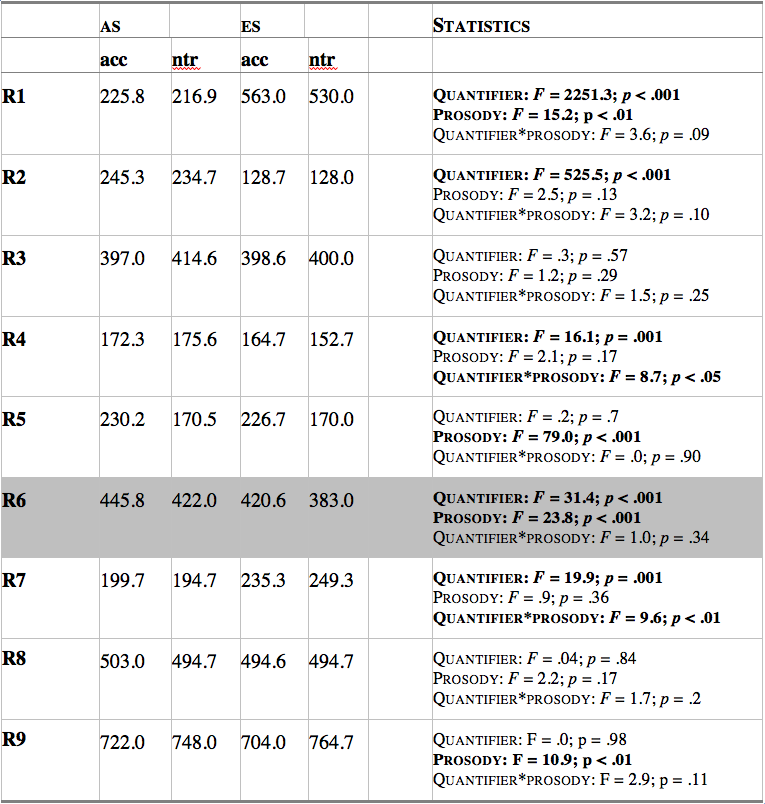
\includegraphics[width=\textwidth]{../pictures/Acoustics/Table-A.png}

  \caption{Durational values in ms for each of the single regions in the target sentences. Region 6 corresponds to \emph{einigen}.}
  \label{tab:table-A}
\end{table}

\begin{table}
  \centering
  
  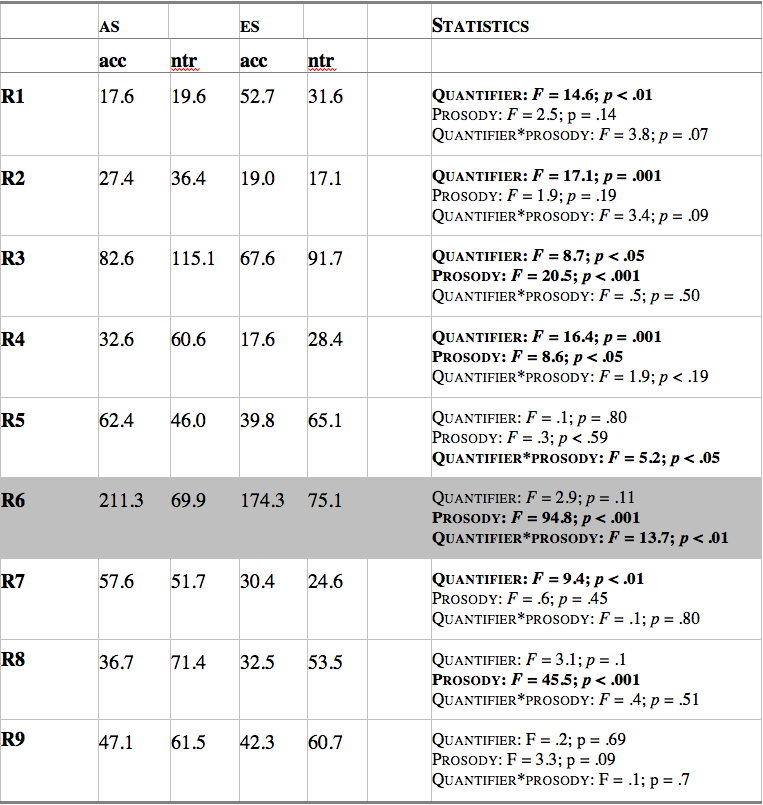
\includegraphics[width=\textwidth]{../pictures/Acoustics/Table-B.png}

  \caption{Difference between minimal and maximal F0 values in Hz for
    each of the single words in the target sentences. Region 6
    corresponds to \emph{einigen}.} 
  \label{tab:table-B}
\end{table}

\paragraph{Target-related fillers.} Table~\ref{tab:table-C} shows the
durational values of each of the single words in the sentence. As is
descriptively evident, the largest durational differences were
realized at the boundary regions (i.e. Region 5 and Region
7). Interestingly, small differences between conditions also yielded
significance at other positions, suggesting that our speaker produced
the different conditions very consistently (i.e., with little
variance).


\begin{table}
  \centering
  
  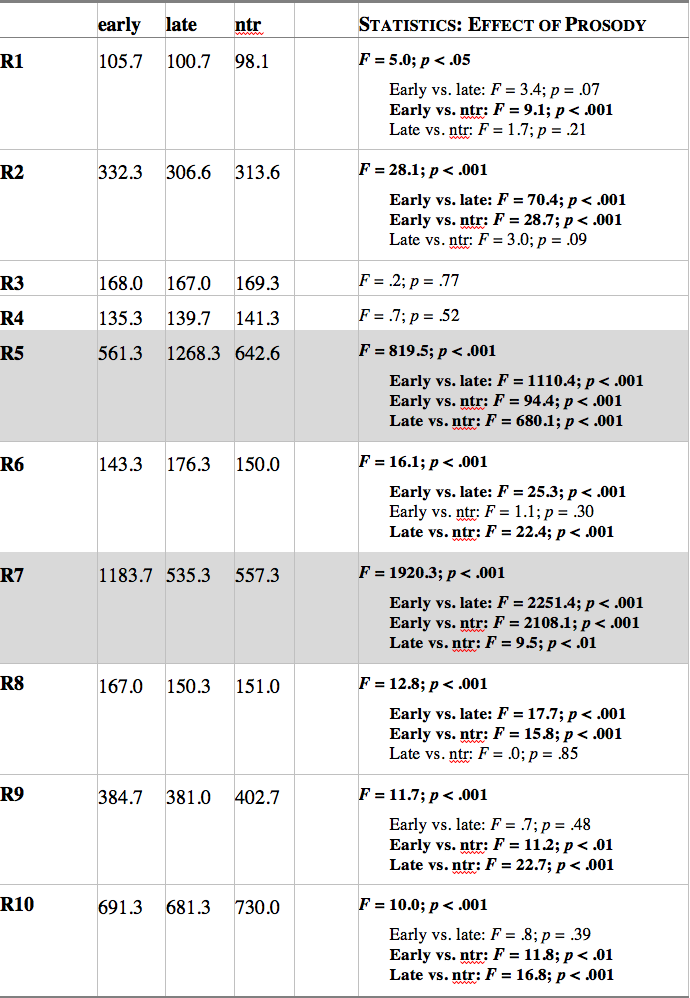
\includegraphics[width=\textwidth]{../pictures/Acoustics/Table-C.png}

  \caption{Durational values in ms for each of the single regions in
    the target-related fillers. Regions 5 and 7 correspond to the
    nouns preceding the boundaries.}  
  \label{tab:table-C}
\end{table}


\begin{table}
  \centering
  
  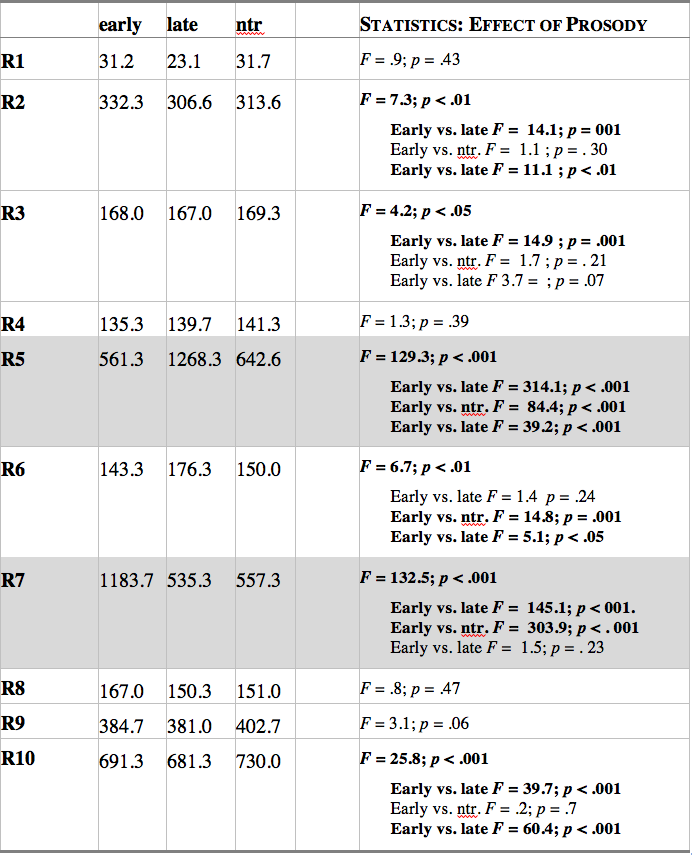
\includegraphics[width=\textwidth]{../pictures/Acoustics/Table-D.png}

  \caption{???}  
  \label{tab:table-D}
\end{table}

\subsection{Participants}
\label{sec:participants} 

41 native speakers of German took part in our study, none of which had
any prior exposure to logic or formal semantics. We excluded 3
subjects due to insufficient performance on controls ($\le 50\%$
correct answers). 

\begin{itemize}
\item possibly mention ages, backgrounds and sexes?
\end{itemize}


\subsection{Results}
\label{sec:results}

The judgments obtained for the four target conditions are depicted in
Figure \ref{fig:JudgmentsK2}.\dn{we should introduce the actual
  sequences that we presented so that it is clear what it means to say
\emph{true} or \emph{false} on some position or other}
%
\begin{figure}[]
\centering
\subfloat[][\as-accented]{
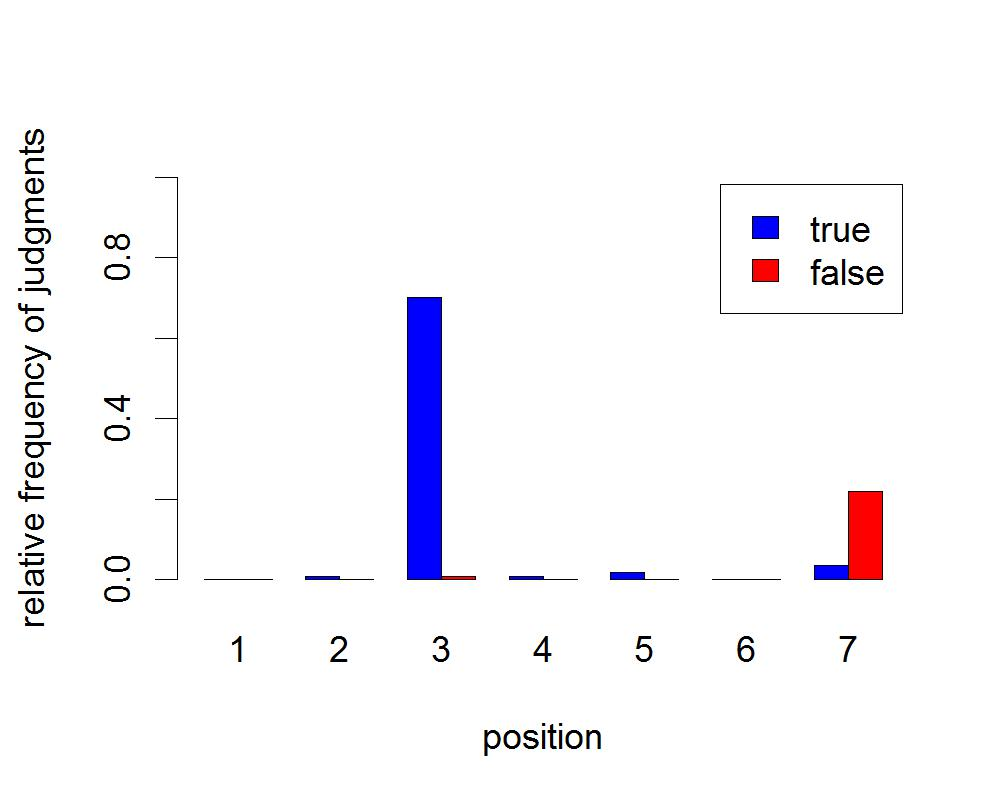
\includegraphics[width=5cm]{../pictures/paper/graph_AE_AKZ.jpg}
\label{fig:ReadingsAE}
}
\subfloat[][\as-neutral]{
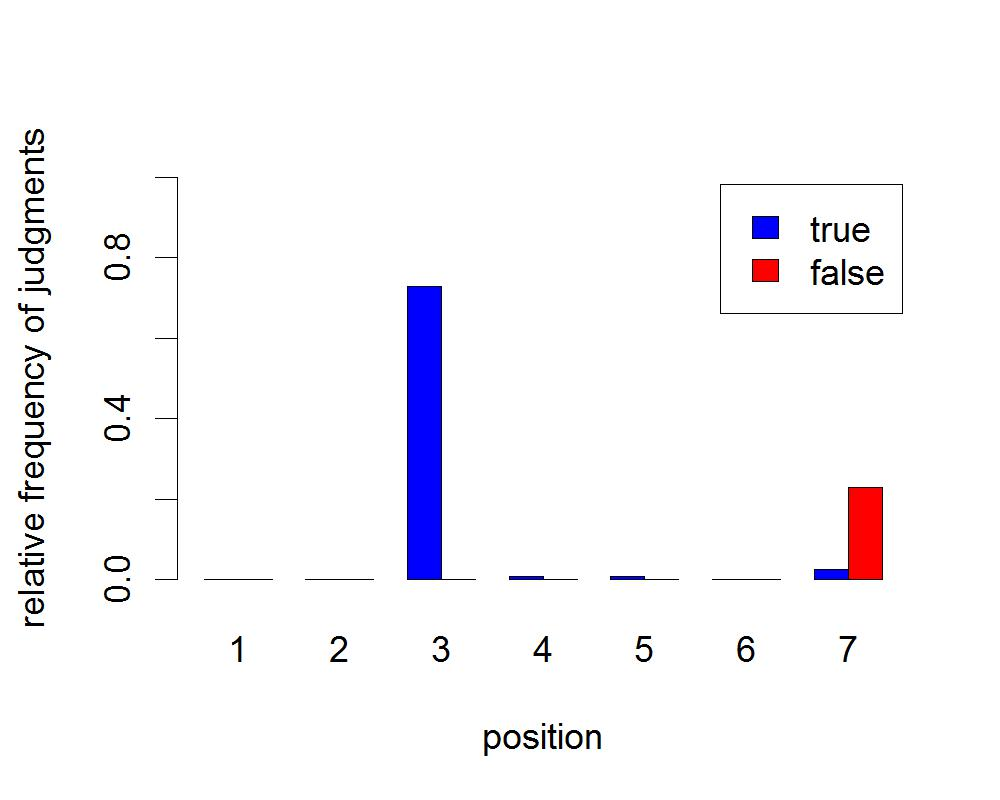
\includegraphics[width=5cm]{../pictures/paper/graph_AE_NTR.jpg}
\label{fig:ReadingsGE}
}

\subfloat[][\es-accented]{
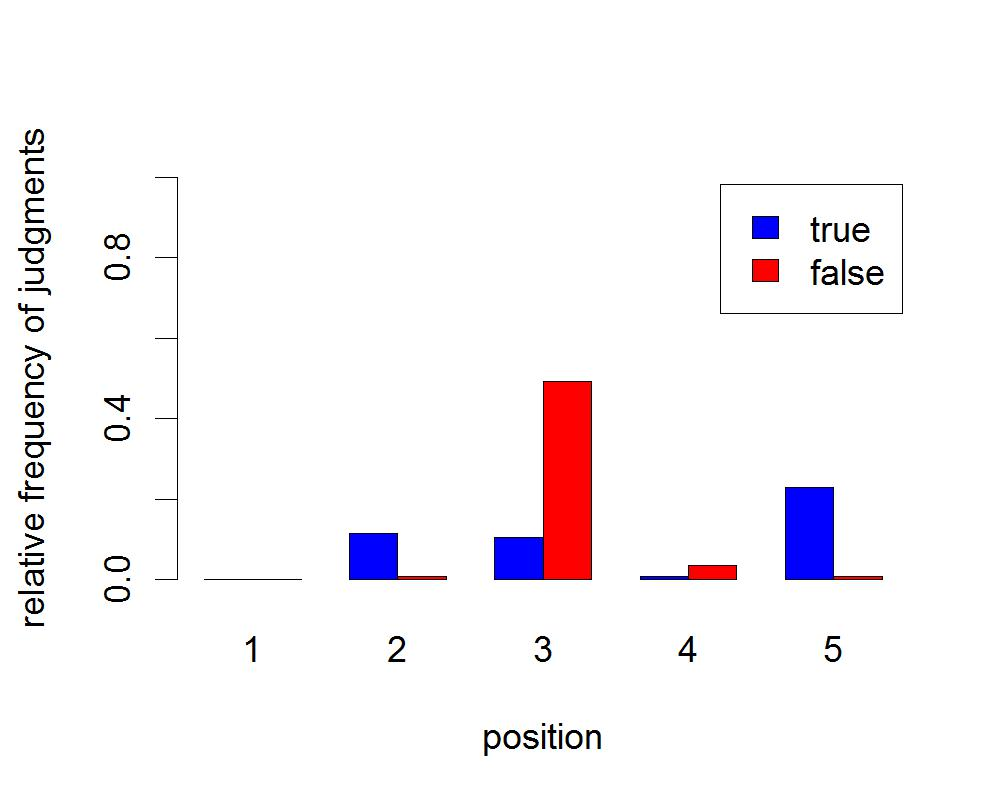
\includegraphics[width=5cm]{../pictures/paper/graph_GE_AKZ.jpg}
\label{fig:ReadingsAE}
}
\subfloat[][\es-neutral]{
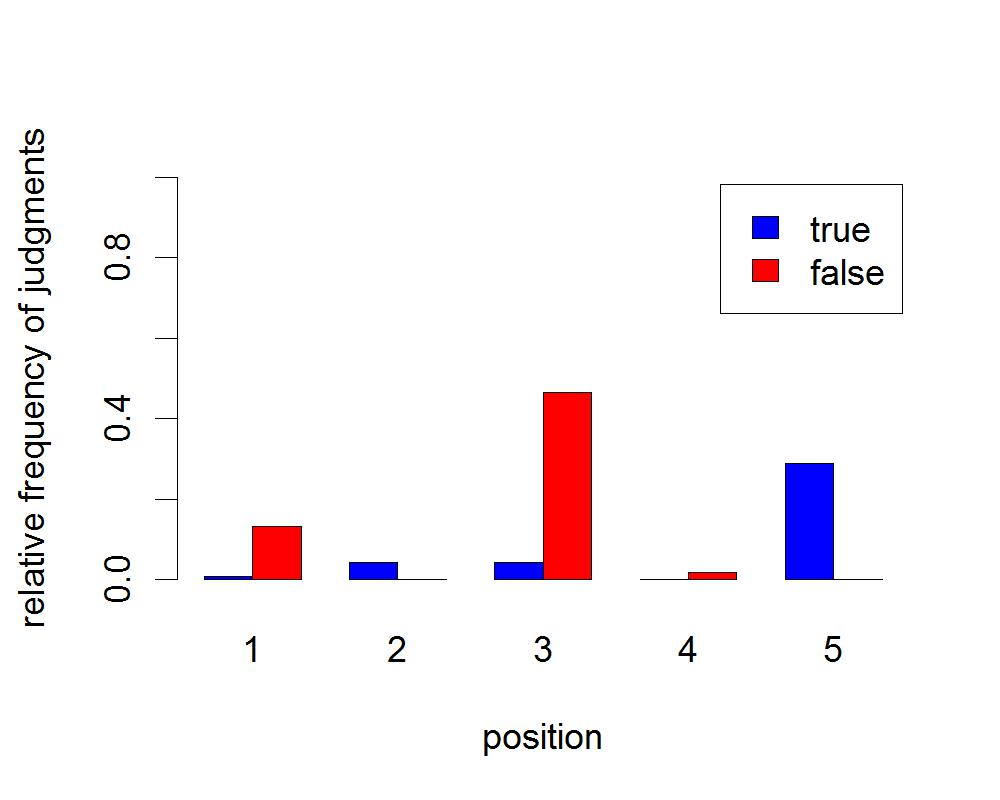
\includegraphics[width=5cm]{../pictures/paper/graph_GE_NTR.jpg}
\label{fig:ReadingsGE}
}

\caption[Optional caption for list of figures]{Judgments for the four
  target conditions in Experiment 1. Relative frequency of
  yes/no-judgments is plotted against the position within the
  trial. In the \as-conditions there were seven positions. On the
  third position a yes-judgment corresponded to a literal reading,
  while on the fith position a yes-judgment corresponded to a global
  reading.  A no-judgment on the seventh position was only consistent
  with a local reading. The \es-conditions had five
  positions. No- judgments on positions two and three corresponded to
  global and literal readings, respectively. A yes-judgment on the
  last segment corresponded to a local reading. }
\label{fig:JudgmentsK2}
\end{figure}
%
We coded the judgments as {\it literal}, {\it global} or {\it local}
if they were as expected under one of these readings and as {\it
  error} if not. The distribution of readings as coded by us is
presented in Figure~\ref{fig:JudgementPercentages}.
%
\begin{figure}[]
\centering
\subfloat[][\as-Conditions]{
\begin{tikzpicture}[scale=0.8]

      \begin{axis}[ybar, 
                  enlarge x limits=0.5,
                  enlarge y limits=0.25,
                  legend style={at={(0.5,-0.15)}, anchor=north, legend columns=-1},
        ylabel={\% of answers}, symbolic x
        coords={ae-ntr,ae-acc}, xtick=data, nodes
        near coords, nodes near coords align={vertical},x=65, bar width=3mm, ymin = 8 ]

        \addplot coordinates {(ae-ntr,73) (ae-acc,70)};

        \addplot coordinates {(ae-ntr,23) (ae-acc,22)};

        \addplot coordinates {(ae-ntr,1) (ae-acc,2)};

        \addplot coordinates {(ae-ntr,4) (ae-acc,6)};

        % \addplot coordinates {(ae-ntr,83) (ae-acc,80) (ge-ntr,53)
        % (ge-acc,56)};

        % \addplot coordinates {(ae-ntr,26) (ae-acc,25) (ge-ntr,33)
        % (ge-acc,26)};

        % \addplot coordinates {(ae-ntr,1) (ae-acc,2) (ge-ntr,0)
        % (ge-acc,1)};

        % \addplot coordinates {(ae-ntr,4) (ae-acc,7) (ge-ntr,28)
        % (ge-acc,31)};

        \legend{literal, local, global, false}

      \end{axis}

    \end{tikzpicture}

% 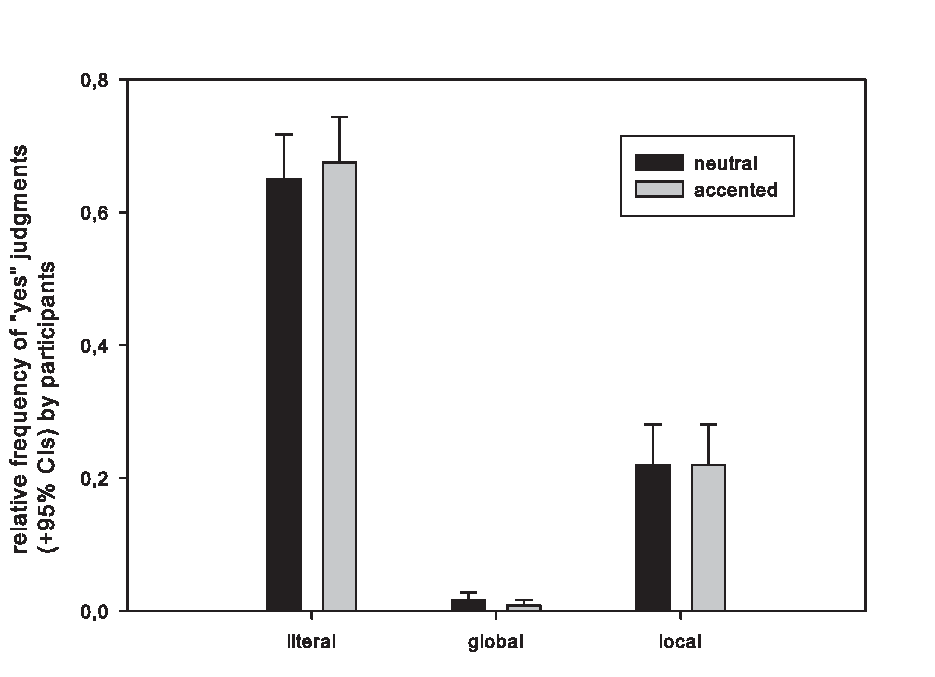
\includegraphics[width=5cm]{../pictures/paper/ReadingsAE.pdf}
\label{fig:JudgementPercentagesAE}
}
\subfloat[][\es-Conditions]{
\begin{tikzpicture}[scale=0.8]

  \begin{axis}[ybar, 
               enlarge x limits=0.5,
               enlarge y limits=0.25, 
               legend style={at={(0.5,-0.15)},
                 anchor=north,
                 legend columns=-1}, 
               ylabel={\% of answers}, 
               symbolic x coords={ge-ntr,ge-acc}, 
               xtick=data,
               nodes near coords,
               nodes near coords align={vertical},
               x=65, bar width=3mm,
               ymin = 8
               ]

    \addplot coordinates {(ge-ntr,47) (ge-acc,49)}; 

    \addplot coordinates {(ge-ntr,29) (ge-acc,23)}; 

    \addplot coordinates {(ge-ntr,0) (ge-acc,1)};

    \addplot coordinates {(ge-ntr,25) (ge-acc,27)};

    % \addplot coordinates {(ae-ntr,83) (ae-acc,80) (ge-ntr,53) (ge-acc,56)}; 

    % \addplot coordinates {(ae-ntr,26) (ae-acc,25) (ge-ntr,33) (ge-acc,26)}; 

    % \addplot coordinates {(ae-ntr,1) (ae-acc,2) (ge-ntr,0) (ge-acc,1)};

    % \addplot coordinates {(ae-ntr,4) (ae-acc,7) (ge-ntr,28) (ge-acc,31)};

    \legend{literal, local, global, false}

  \end{axis}

\end{tikzpicture}

% 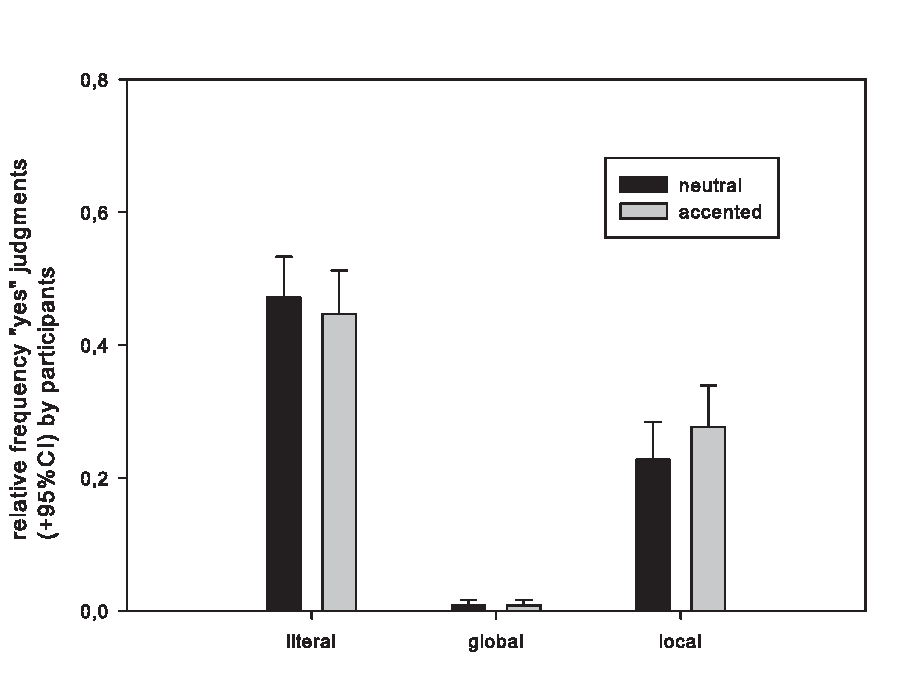
\includegraphics[width=5cm]{../pictures/paper/ReadingsGE.pdf}
\label{fig:JudgementPercentagesGE}
}
\caption[Optional caption for list of figures]{Judgments}
\label{fig:JudgementPercentages}
\end{figure}
%
Participants mostly gave judgments indicating literal or local
readings. Judgments compatible with a global reading were seldom
obtained. In the \as-conditions participants made hardly any errors,
whereas the amount of errors was slightly greater in the
\es-conditions.

In the \as-conditions (see Figure~\ref{fig:JudgementPercentagesAE})
judgments were consistent with literal readings in 65.0\% of the
trials with neutral prosody and in 67.5\% of the trials with accented
prosody.\dn{IMPORTANT: Figure contains different numbers (even if
  rounded)! Fabian, did you exclude the 3 bad performers when you
  obtained this data?} The number of global readings was very low,
with 1.6\% of the neutral and 0.8\% of the accented trials
(corresponding to a total of 3 answers across all trials). Judgments
indicating local readings were given in 22.0\% of both the neutral and
accented trials. In the \es-conditions (see
Figure~\ref{fig:JudgementPercentagesGE}) judgments consistent with
literal readings were given in 47.2\% and 44.7\% of the trials with
neutral and accented prosody, respectively. Global readings were
observed in 0.8\% of the trials in both the neutral and the accented
condition. Judgments indicating local readings were given in 22.8\% of
the neutral and 27.6\% of the accented trials.

In order to test wether local readings exist we tested whether the
number of local responses in each condition was higher than expected
by chance. Local responses had to be given on the last position in
each trial. If local readings didn't exist we would expect
participants, who reached the last position (ie. who did not abort the
trial prior to the last position) to give local judgments not more
often than expected by chance. On the last position two responses were
possible. One was compatible with a local reading the other was
not. Therefore, we would expect 50\% local responses by chance. As it
turns out local responses were given significantly more often than
50\% in all target conditions (all Bonferoni corrected p<.05). Note
that this finding cannot be explained by some kind of general response
bias on the last position since local readings required a yes-judgment
in the \es-conditions but a no-judgment in the \as-conditions.

In order to test whether accentuation or the quantifier has an
influence on the distribution of readings, log-liner models were
computed (see Schepers 2003). The factors {\it Reading}, {\it
  Accentuation} and {\it Quantifier} were included in these
models. Two variants of these models were computed.  In the first, the
factor {\it Item} was added to the above mentioned. In the latter {\it
  Participants} was included as a factor. Inclusion of these two
factors allowed us to test whether the distribution of readings was
identical accros items and participants. We report log-likelihood
ratio Chi-squares ($LRCS_1$ and $LRCS_2$), degrees of freedom ($df_1$,
$df_2$) and significance levels ($p_1$ and $p_2$).

Unsurprisingly, there was an effect of reading ($LRCS_1=364.77, df_1 =
3, p_1<.001, LRCS_2=364.77, df_2 = 3, p_1<.001,$) because overall the
readings were distributed inhomogeneously (sse Figure
\ref{fig:ReadingsGE}). The quantifier had an influence on the
distribution of readings as revealed by a reliable interaction of {\it
  Reading} and {\it Quantifier} ($LRCS_1=49.32, p_1<.01,LRCS_2=32.16,
p_1<.01,$). Looking at the data it seemed unlikely that the quantifier
affected the amount of local readings. We suspected that this
interaction was due to the higher number of errors and lower number of
literal readings in the \es-conditions as compared with
the \as-conditions. A difference in the distribution of judgment
types between participants was revealed by a reliable interaction of
{\it Reading} and {\it Participant} ($LRCS_1=487.70, p_1<.01$). We
were interested in whether this effect was due to some of the
participants being more likely to choose literal readings than
others. Finally, there was a three-way interaction of {\it
  Participants}, {\it Construction} and {\it Reading} ($LRCS_1, =
143.92, df_1 = 117, p_1<.05$) which could stem from to the fact that
some participants were more prone than others to make errors in the
\es-conditions.

In order to find out whether the interactions just reported affected
the amount of local readings, the log-linear models were computed
again with a different coding of the readings. Here, we only
considered the amount of local readings versus all other kinds of
judgments. Judgments were coded as {\it local} and {\it other}. If the
reported interactions affect the amount of local readings they should
show up again. The expected but irrelevant effect of {\it Reading} was
again significant ($LRCS_1=134.55, df_1 = 1, p_1<.001, LRCS_2=144.64,
df_2 = 1, p_1<.001,$). In addition, the interaction of {\it
  Participant} and {\it Reading} ($LRCS_1=487.70, p_1<.01$) as well as
the three-way interaction of {\it Construction}, {\it Participant} and
{\it Reading} ($LRCS_1=487.70, p_1<.01$) were significant. No other
effects were significant. In particular, the interaction of {\it
  Construction} and {\it Reading} was not significant ($LRCS_1=2.10,
p_1=.15,LRCS_2=.74, p_2=.39$).

The interaction of {\it Participant} and {\it Reading} shows that
there are indeed varying preferences for local readings among German
speakers. Further examination of the distribution of local readings
revealed a clear pattern (see Figure
\ref{fig:HistogramLocalReadingsK2}). In all four conditions, about
seven out of the 40 participants ($16\%$) were consistently giving
judgments that indicate local readings. Further, the relative
frequency of local judgments per participant strongly correlated
between all four conditions (all $r>.6, p<.001$). Appart from the
localists about half of the participants (and 41.5\% of all
participants) were consistently giving judgments that indicate literal
readings. Only a minority of participants exhibited
inconsistency. Reading preferences were more clear-cut in the
\as-conditions than in the \es-conditions. The number of consistent
litaralists was lower in the \es-conditions (25.6\%) as compared to
the \as-conditions (57.3\%). Also, the number of participants that
showed inconsitency was higher in these conditions. However, the
number of consistent localists did hardly differ between
constructions.

The three way-interaction of {\it Participant}, {\it Construction} and
{\it Reading} is due to the fact that for some participants
preferences for local over other readings deviated between the two
construction types. These deviations were, however, not systematic to
any degree. How much local preferences deviated between the two
construction types per participant is depicted in Figure \ref{}. Most
participants had exactly the same preferences in the two
constructions. However, a few had a stronger and a few others a weaker
preference for local readings in the \es- than in the
\as-conditions. Since we did not find any systematic patterns
here, we speculate that the three-way interaction is due to the
\es-construction beeing understood non-standardly by a
few participants. This speculation is plausible given the higher
number of errors in the \es- as compared to the \as-conditions.

The absence of the interaction between {\it Construction} and {\it
  Participant} indicates that the type of construction does not affect
the amount of local readings. We assumed based on the observed
distribution of judgments that the type of contsruction affected the
amount of literal but not local and global readings. To further test
this assumption, we also considered literal and global readings versus
other judgments in separate analyses. Comparing global readings versus
other judgments {\it Construction} and {\it Reading} were found to
interact ($LRCS_1=42.80, df= 1, p<.001; LRCS_2=22.14, df= 1,
p<.001$). Comparing global readings to other judgments no such
interaction was obeserved ($LRCS_1=1.24, df= 1, p=.29, LRCS_1=.21, df=
1, p=.65$).

 


\begin{figure}[h]
\centering
\subfloat[][\as-accented]{
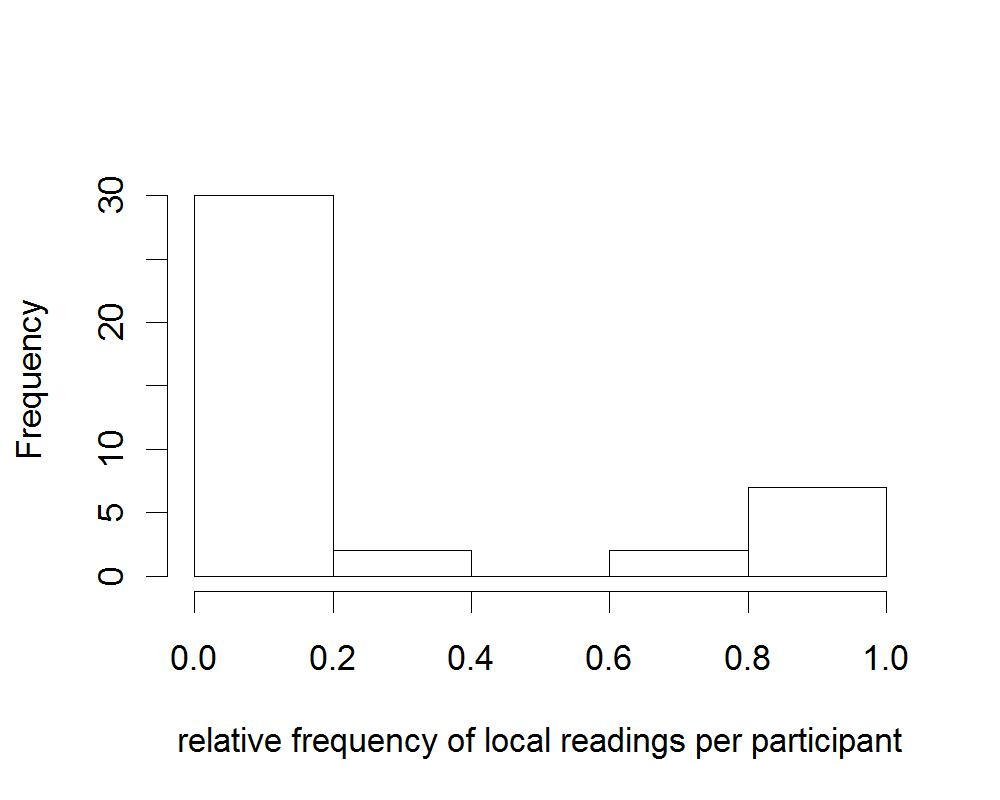
\includegraphics[width=5cm]{../pictures/paper/histLocalReadingAE_AKZ.jpg}
\label{fig:ReadingsAE}
}
\subfloat[][\as-neutral]{
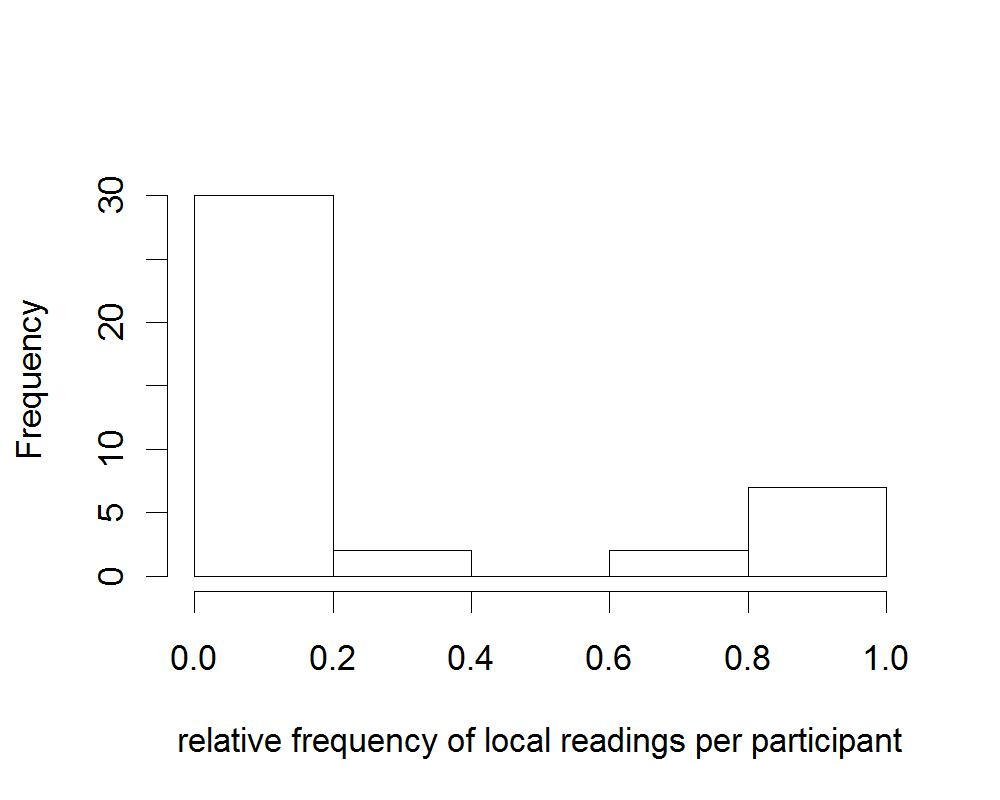
\includegraphics[width=5cm]{../pictures/paper/histLocalReadingAE_NTR.jpg}
\label{fig:ReadingsGE}
}

\subfloat[][\es-accented]{
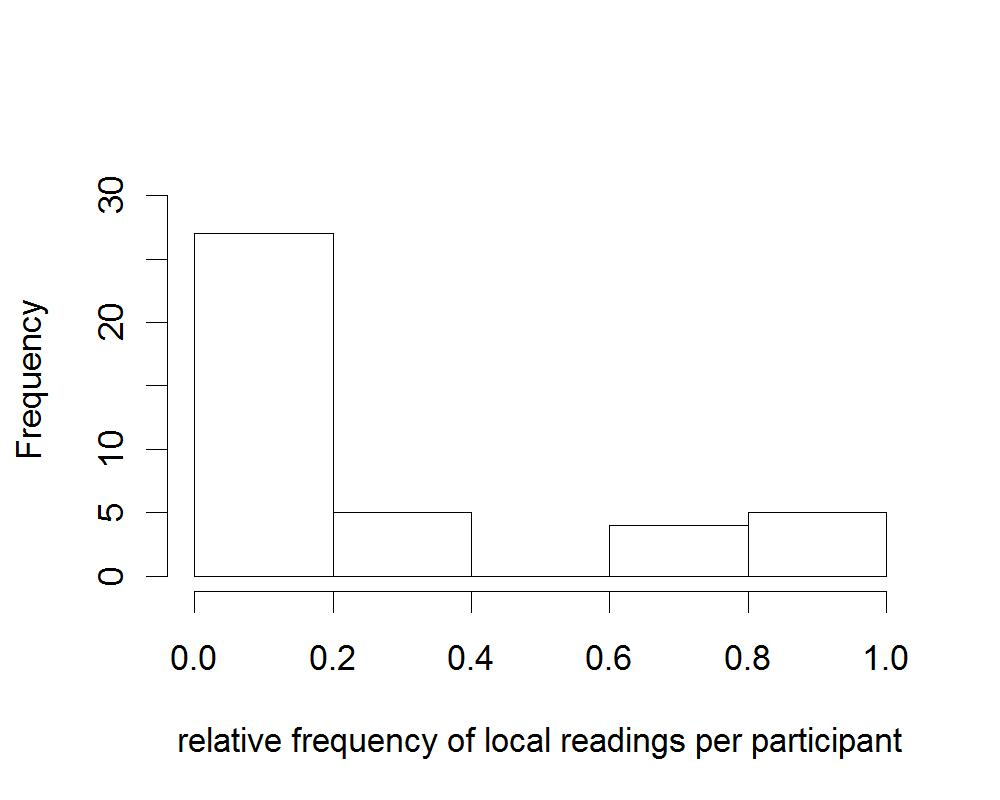
\includegraphics[width=5cm]{../pictures/paper/histLocalReadingGE_AKZ.jpg}
\label{fig:ReadingsAE}
}
\subfloat[][\es-neutral]{
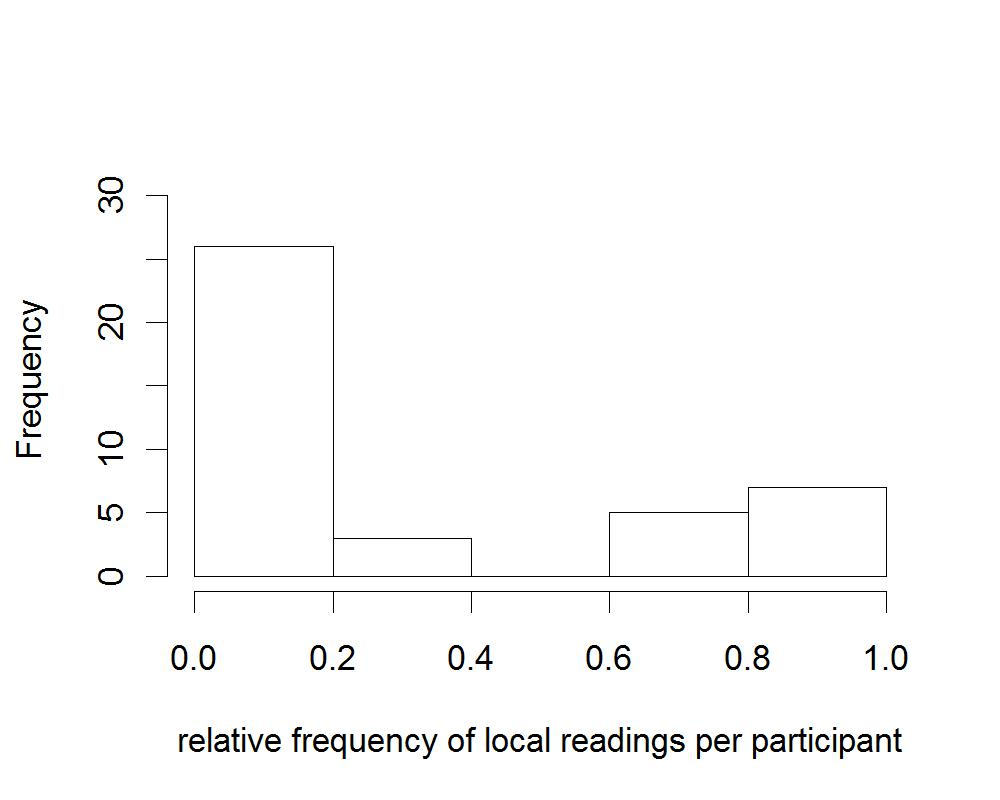
\includegraphics[width=5cm]{../pictures/paper/histLocalReadingGE_NTR.jpg}
\label{fig:ReadingsGE}
}
\label{fig:HistogramLocalReadingsK2}
\caption[Optional caption for list of figures]{Judgments for the four target conditions}
\end{figure}

\subsection{Discussion}
\label{sec:discussion}

\lipsum[1]

\section{Conclusions}
\label{sec:conclusions}



\printbibliography[heading=bibintoc]

\end{document}
